\documentclass[journal,12pt,twocolumn]{IEEEtran}
%
\usepackage{setspace}
\usepackage{gensymb}
%\doublespacing
\singlespacing

%\usepackage{graphicx}
%\usepackage{amssymb}
%\usepackage{relsize}
\usepackage[cmex10]{amsmath}
%\usepackage{amsthm}
%\interdisplaylinepenalty=2500
%\savesymbol{iint}
%\usepackage{txfonts}
%\restoresymbol{TXF}{iint}
%\usepackage{wasysym}
\usepackage{amsthm}
%\usepackage{iithtlc}
\usepackage{mathrsfs}
\usepackage{txfonts}
\usepackage{stfloats}
\usepackage{bm}
\usepackage{cite}
\usepackage{cases}
\usepackage{subfig}
%\usepackage{xtab}
\usepackage{longtable}
\usepackage{multirow}
%\usepackage{algorithm}
%\usepackage{algpseudocode}
\usepackage{enumitem}
\usepackage{mathtools}
\usepackage{steinmetz}
\usepackage{tikz}
\usepackage[american]{circuitikz}
\usepackage{verbatim}
\usepackage{tfrupee}
\usepackage[breaklinks=true]{hyperref}
%\usepackage{stmaryrd}
\usepackage{tkz-euclide} % loads  TikZ and tkz-base
\usetkzobj{all}
\usetikzlibrary{decorations.markings}
\usetikzlibrary{shapes.geometric}
\usetikzlibrary{positioning, fit, calc}
\newif\iflabrev
\usepackage{listings}
    \usepackage{color}                                            %%
    \usepackage{array}                                            %%
    \usepackage{longtable}                                        %%
    \usepackage{calc}                                             %%
    \usepackage{multirow}                                         %%
    \usepackage{hhline}                                           %%
    \usepackage{ifthen}                                           %%
  %optionally (for landscape tables embedded in another document): %%
    \usepackage{lscape}     
\usepackage{multicol}
\usepackage{chngcntr}
%\usepackage{enumerate}

%\usepackage{wasysym}
%\newcounter{MYtempeqncnt}
\DeclareMathOperator*{\Res}{Res}
%\renewcommand{\baselinestretch}{2}
\renewcommand\thesection{\arabic{section}}
\renewcommand\thesubsection{\thesection.\arabic{subsection}}
\renewcommand\thesubsubsection{\thesubsection.\arabic{subsubsection}}

\renewcommand\thesectiondis{\arabic{section}}
\renewcommand\thesubsectiondis{\thesectiondis.\arabic{subsection}}
\renewcommand\thesubsubsectiondis{\thesubsectiondis.\arabic{subsubsection}}

% correct bad hyphenation here
\hyphenation{op-tical net-works semi-conduc-tor}
\def\inputGnumericTable{}                                 %%

\lstset{
%language=C,
frame=single, 
breaklines=true,
columns=fullflexible
}
%\lstset{
%language=tex,
%frame=single, 
%breaklines=true
%}

\begin{document}
%


\newtheorem{theorem}{Theorem}[section]
\newtheorem{problem}{Problem}
\newtheorem{proposition}{Proposition}[section]
\newtheorem{lemma}{Lemma}[section]
\newtheorem{corollary}[theorem]{Corollary}
\newtheorem{example}{Example}[section]
\newtheorem{definition}[problem]{Definition}
%\newtheorem{thm}{Theorem}[section] 
%\newtheorem{defn}[thm]{Definition}
%\newtheorem{algorithm}{Algorithm}[section]
%\newtheorem{cor}{Corollary}
\newcommand{\BEQA}{\begin{eqnarray}}
\newcommand{\EEQA}{\end{eqnarray}}
\newcommand{\define}{\stackrel{\triangle}{=}}

\bibliographystyle{IEEEtran}
%\bibliographystyle{ieeetr}


\providecommand{\mbf}{\mathbf}
\providecommand{\pr}[1]{\ensuremath{\Pr\left(#1\right)}}
\providecommand{\qfunc}[1]{\ensuremath{Q\left(#1\right)}}
\providecommand{\sbrak}[1]{\ensuremath{{}\left[#1\right]}}
\providecommand{\lsbrak}[1]{\ensuremath{{}\left[#1\right.}}
\providecommand{\rsbrak}[1]{\ensuremath{{}\left.#1\right]}}
\providecommand{\brak}[1]{\ensuremath{\left(#1\right)}}
\providecommand{\lbrak}[1]{\ensuremath{\left(#1\right.}}
\providecommand{\rbrak}[1]{\ensuremath{\left.#1\right)}}
\providecommand{\cbrak}[1]{\ensuremath{\left\{#1\right\}}}
\providecommand{\lcbrak}[1]{\ensuremath{\left\{#1\right.}}
\providecommand{\rcbrak}[1]{\ensuremath{\left.#1\right\}}}
\theoremstyle{remark}
\newtheorem{rem}{Remark}
\newcommand{\sgn}{\mathop{\mathrm{sgn}}}
\providecommand{\abs}[1]{\left\vert#1\right\vert}
\providecommand{\res}[1]{\Res\displaylimits_{#1}} 
\providecommand{\norm}[1]{\left\lVert#1\right\rVert}
%\providecommand{\norm}[1]{\lVert#1\rVert}
\providecommand{\mtx}[1]{\mathbf{#1}}
\providecommand{\mean}[1]{E\left[ #1 \right]}
\providecommand{\fourier}{\overset{\mathcal{F}}{ \rightleftharpoons}}
%\providecommand{\hilbert}{\overset{\mathcal{H}}{ \rightleftharpoons}}
\providecommand{\system}{\overset{\mathcal{H}}{ \longleftrightarrow}}
	%\newcommand{\solution}[2]{\textbf{Solution:}{#1}}
\newcommand{\solution}{\noindent \textbf{Solution: }}
\newcommand{\cosec}{\,\text{cosec}\,}
\providecommand{\dec}[2]{\ensuremath{\overset{#1}{\underset{#2}{\gtrless}}}}
\newcommand{\myvec}[1]{\ensuremath{\begin{pmatrix}#1\end{pmatrix}}}
\newcommand{\mydet}[1]{\ensuremath{\begin{vmatrix}#1\end{vmatrix}}}
%\numberwithin{equation}{section}
\numberwithin{equation}{subsection}
%\numberwithin{problem}{section}
%\numberwithin{definition}{section}
\makeatletter
\@addtoreset{figure}{problem}
\makeatother

\let\StandardTheFigure\thefigure
\let\vec\mathbf
%\renewcommand{\thefigure}{\theproblem.\arabic{figure}}
\renewcommand{\thefigure}{\theproblem}
%\setlist[enumerate,1]{before=\renewcommand\theequation{\theenumi.\arabic{equation}}
%\counterwithin{equation}{enumi}


%\renewcommand{\theequation}{\arabic{subsection}.\arabic{equation}}

\def\putbox#1#2#3{\makebox[0in][l]{\makebox[#1][l]{}\raisebox{\baselineskip}[0in][0in]{\raisebox{#2}[0in][0in]{#3}}}}
     \def\rightbox#1{\makebox[0in][r]{#1}}
     \def\centbox#1{\makebox[0in]{#1}}
     \def\topbox#1{\raisebox{-\baselineskip}[0in][0in]{#1}}
     \def\midbox#1{\raisebox{-0.5\baselineskip}[0in][0in]{#1}}

\vspace{3cm}

\title{
%	\logo{
Control Systems
%	}
}
\author{ G V V Sharma$^{*}$% <-this % stops a space
	\thanks{*The author is with the Department
		of Electrical Engineering, Indian Institute of Technology, Hyderabad
		502285 India e-mail:  gadepall@iith.ac.in. All content in this manual is released under GNU GPL.  Free and open source.}
	
}	
%\title{
%	\logo{Matrix Analysis through Octave}{\begin{center}\includegraphics[scale=.24]{tlc}\end{center}}{}{HAMDSP}
%}


% paper title
% can use linebreaks \\ within to get better formatting as desired
%\title{Matrix Analysis through Octave}
%
%
% author names and IEEE memberships
% note positions of commas and nonbreaking spaces ( ~ ) LaTeX will not break
% a structure at a ~ so this keeps an author's name from being broken across
% two lines.
% use \thanks{} to gain access to the first footnote area
% a separate \thanks must be used for each paragraph as LaTeX2e's \thanks
% was not built to handle multiple paragraphs
%

%\author{<-this % stops a space
%\thanks{}}
%}
% note the % following the last \IEEEmembership and also \thanks - 
% these prevent an unwanted space from occurring between the last author name
% and the end of the author line. i.e., if you had this:
% 
% \author{....lastname \thanks{...} \thanks{...} }
%                     ^------------^------------^----Do not want these spaces!
%
% a space would be appended to the last name and could cause every name on that
% line to be shifted left slightly. This is one of those "LaTeX things". For
% instance, "\textbf{A} \textbf{B}" will typeset as "A B" not "AB". To get
% "AB" then you have to do: "\textbf{A}\textbf{B}"
% \thanks is no different in this regard, so shield the last } of each \thanks
% that ends a line with a % and do not let a space in before the next \thanks.
% Spaces after \IEEEmembership other than the last one are OK (and needed) as
% you are supposed to have spaces between the names. For what it is worth,
% this is a minor point as most people would not even notice if the said evil
% space somehow managed to creep in.



% The paper headers
%\markboth{Journal of \LaTeX\ Class Files,~Vol.~6, No.~1, January~2007}%
%{Shell \MakeLowercase{\textit{et al.}}: Bare Demo of IEEEtran.cls for Journals}
% The only time the second header will appear is for the odd numbered pages
% after the title page when using the twoside option.
% 
% *** Note that you probably will NOT want to include the author's ***
% *** name in the headers of peer review papers.                   ***
% You can use \ifCLASSOPTIONpeerreview for conditional compilation here if
% you desire.




% If you want to put a publisher's ID mark on the page you can do it like
% this:
%\IEEEpubid{0000--0000/00\$00.00~\copyright~2007 IEEE}
% Remember, if you use this you must call \IEEEpubidadjcol in the second
% column for its text to clear the IEEEpubid mark.



% make the title area
\maketitle

\newpage

\tableofcontents

\bigskip

\renewcommand{\thefigure}{\theenumi}
\renewcommand{\thetable}{\theenumi}
%\renewcommand{\theequation}{\theenumi}

%\begin{abstract}
%%\boldmath
%In this letter, an algorithm for evaluating the exact analytical bit error rate  (BER)  for the piecewise linear (PL) combiner for  multiple relays is presented. Previous results were available only for upto three relays. The algorithm is unique in the sense that  the actual mathematical expressions, that are prohibitively large, need not be explicitly obtained. The diversity gain due to multiple relays is shown through plots of the analytical BER, well supported by simulations. 
%
%\end{abstract}
% IEEEtran.cls defaults to using nonbold math in the Abstract.
% This preserves the distinction between vectors and scalars. However,
% if the journal you are submitting to favors bold math in the abstract,
% then you can use LaTeX's standard command \boldmath at the very start
% of the abstract to achieve this. Many IEEE journals frown on math
% in the abstract anyway.

% Note that keywords are not normally used for peerreview papers.
%\begin{IEEEkeywords}
%Cooperative diversity, decode and forward, piecewise linear
%\end{IEEEkeywords}



% For peer review papers, you can put extra information on the cover
% page as needed:
% \ifCLASSOPTIONpeerreview
% \begin{center} \bfseries EDICS Category: 3-BBND \end{center}
% \fi
%
% For peerreview papers, this IEEEtran command inserts a page break and
% creates the second title. It will be ignored for other modes.
%\IEEEpeerreviewmaketitle

\begin{abstract}
This manual is an introduction to control systems in feedback circuits. Links to sample Python codes are available in the text.  
\end{abstract}
Download python codes using 
\begin{lstlisting}
svn co https://github.com/gadepall/school/trunk/control/feedback/codes
\end{lstlisting}

\section{Feedback Voltage Amplifier: Series-Shunt}
%\begin{enumerate}[label=\thesection.\arabic*.,ref=\thesection.\theenumi]
\numberwithin{equation}{enumi}

\item Fig. \ref{fig:ee18btech11005_original_circuit} shows a  non-inverting op-amp configuration   with parameters described in Table \ref{table:ee18btech11005_Input_Table}.  Draw the equivalent control system.
\renewcommand{\thefigure}{\theenumi.\arabic{figure}}
%
\begin{figure}[!ht]
	\begin{center}
		
		\resizebox{\columnwidth}{!}{\begin{circuitikz}
\ctikzset{bipoles/length=1cm}

\draw 
(0, 0) node[op amp] (opamp) {}
(opamp.-) to[R,l_=$R_1$,*-*] (-2, 0.35) to (-2.5, 0.35) to (-2.5, 0.35) node[ground]{}
(opamp.-) --(-0.9,1) to[R=$R_2$] (1,1) -- (1,0) --(2,0) node at(2.3,0){$V_0$}
(opamp.out) to (1.5,0)--(1.5,-0.5) to[R=$R_L$] (1.5,-1.5) to (1.5,-1.5) node[ground]{}
(opamp.+) -- (-0.6,-0.35) to[R =$R_s$,*-*] (-2.6,-0.35) to[V=$V_s$] (-2.6,-2.4) node[ground]{}
;\end{circuitikz}
}
	\end{center}
\caption{}
\label{fig:ee18btech11005_original_circuit}
\end{figure}
%
\begin{table}[!ht]
\centering

%%%%%%%%%%%%%%%%%%%%%%%%%%%%%%%%%%%%%%%%%%%%%%%%%%%%%%%%%%%%%%%%%%%%%%
%%                                                                  %%
%%  This is the header of a LaTeX2e file exported from Gnumeric.    %%
%%                                                                  %%
%%  This file can be compiled as it stands or included in another   %%
%%  LaTeX document. The table is based on the longtable package so  %%
%%  the longtable options (headers, footers...) can be set in the   %%
%%  preamble section below (see PRAMBLE).                           %%
%%                                                                  %%
%%  To include the file in another, the following two lines must be %%
%%  in the including file:                                          %%
%%        \def\inputGnumericTable{}                                 %%
%%  at the beginning of the file and:                               %%
%%        \input{name-of-this-file.tex}                             %%
%%  where the table is to be placed. Note also that the including   %%
%%  file must use the following packages for the table to be        %%
%%  rendered correctly:                                             %%
%%    \usepackage[latin1]{inputenc}                                 %%
%%    \usepackage{color}                                            %%
%%    \usepackage{array}                                            %%
%%    \usepackage{longtable}                                        %%
%%    \usepackage{calc}                                             %%
%%    \usepackage{multirow}                                         %%
%%    \usepackage{hhline}                                           %%
%%    \usepackage{ifthen}                                           %%
%%  optionally (for landscape tables embedded in another document): %%
%%    \usepackage{lscape}                                           %%
%%                                                                  %%
%%%%%%%%%%%%%%%%%%%%%%%%%%%%%%%%%%%%%%%%%%%%%%%%%%%%%%%%%%%%%%%%%%%%%%



%%  This section checks if we are begin input into another file or  %%
%%  the file will be compiled alone. First use a macro taken from   %%
%%  the TeXbook ex 7.7 (suggestion of Han-Wen Nienhuys).            %%
\def\ifundefined#1{\expandafter\ifx\csname#1\endcsname\relax}


%%  Check for the \def token for inputed files. If it is not        %%
%%  defined, the file will be processed as a standalone and the     %%
%%  preamble will be used.                                          %%
\ifundefined{inputGnumericTable}

%%  We must be able to close or not the document at the end.        %%
	\def\gnumericTableEnd{\end{document}}


%%%%%%%%%%%%%%%%%%%%%%%%%%%%%%%%%%%%%%%%%%%%%%%%%%%%%%%%%%%%%%%%%%%%%%
%%                                                                  %%
%%  This is the PREAMBLE. Change these values to get the right      %%
%%  paper size and other niceties.                                  %%
%%                                                                  %%
%%%%%%%%%%%%%%%%%%%%%%%%%%%%%%%%%%%%%%%%%%%%%%%%%%%%%%%%%%%%%%%%%%%%%%

	\documentclass[12pt%
			  %,landscape%
                    ]{report}
       \usepackage[latin1]{inputenc}
       \usepackage{fullpage}
       \usepackage{color}
       \usepackage{array}
       \usepackage{longtable}
       \usepackage{calc}
       \usepackage{multirow}
       \usepackage{hhline}
       \usepackage{ifthen}



%%  End of the preamble for the standalone. The next section is for %%
%%  documents which are included into other LaTeX2e files.          %%
\else

%%  We are not a stand alone document. For a regular table, we will %%
%%  have no preamble and only define the closing to mean nothing.   %%
    \def\gnumericTableEnd{}

%%  If we want landscape mode in an embedded document, comment out  %%
%%  the line above and uncomment the two below. The table will      %%
%%  begin on a new page and run in landscape mode.                  %%
%       \def\gnumericTableEnd{\end{landscape}}
%       \begin{landscape}


%%  End of the else clause for this file being \input.              %%
\fi

%%%%%%%%%%%%%%%%%%%%%%%%%%%%%%%%%%%%%%%%%%%%%%%%%%%%%%%%%%%%%%%%%%%%%%
%%                                                                  %%
%%  The rest is the gnumeric table, except for the closing          %%
%%  statement. Changes below will alter the table's appearance.     %%
%%                                                                  %%
%%%%%%%%%%%%%%%%%%%%%%%%%%%%%%%%%%%%%%%%%%%%%%%%%%%%%%%%%%%%%%%%%%%%%%

\providecommand{\gnumericmathit}[1]{#1} 
%%  Uncomment the next line if you would like your numbers to be in %%
%%  italics if they are italizised in the gnumeric table.           %%
%\renewcommand{\gnumericmathit}[1]{\mathit{#1}}
\providecommand{\gnumericPB}[1]%
{\let\gnumericTemp=\\#1\let\\=\gnumericTemp\hspace{0pt}}
 \ifundefined{gnumericTableWidthDefined}
        \newlength{\gnumericTableWidth}
        \newlength{\gnumericTableWidthComplete}
        \newlength{\gnumericMultiRowLength}
        \global\def\gnumericTableWidthDefined{}
 \fi
%% The following setting protects this code from babel shorthands.  %%
 \ifthenelse{\isundefined{\languageshorthands}}{}{\languageshorthands{english}}
%%  The default table format retains the relative column widths of  %%
%%  gnumeric. They can easily be changed to c, r or l. In that case %%
%%  you may want to comment out the next line and uncomment the one %%
%%  thereafter                                                      %%
\providecommand\gnumbox{\makebox[0pt]}
%%\providecommand\gnumbox[1][]{\makebox}

%% to adjust positions in multirow situations                       %%
\setlength{\bigstrutjot}{\jot}
\setlength{\extrarowheight}{\doublerulesep}

%%  The \setlongtables command keeps column widths the same across  %%
%%  pages. Simply comment out next line for varying column widths.  %%
\setlongtables

\setlength\gnumericTableWidth{%
	53pt+%
	93pt+%
0pt}
\def\gumericNumCols{2}
\setlength\gnumericTableWidthComplete{\gnumericTableWidth+%
         \tabcolsep*\gumericNumCols*2+\arrayrulewidth*\gumericNumCols}
\ifthenelse{\lengthtest{\gnumericTableWidthComplete > \linewidth}}%
         {\def\gnumericScale{\ratio{\linewidth-%
                        \tabcolsep*\gumericNumCols*2-%
                        \arrayrulewidth*\gumericNumCols}%
{\gnumericTableWidth}}}%
{\def\gnumericScale{1}}

%%%%%%%%%%%%%%%%%%%%%%%%%%%%%%%%%%%%%%%%%%%%%%%%%%%%%%%%%%%%%%%%%%%%%%
%%                                                                  %%
%% The following are the widths of the various columns. We are      %%
%% defining them here because then they are easier to change.       %%
%% Depending on the cell formats we may use them more than once.    %%
%%                                                                  %%
%%%%%%%%%%%%%%%%%%%%%%%%%%%%%%%%%%%%%%%%%%%%%%%%%%%%%%%%%%%%%%%%%%%%%%

\ifthenelse{\isundefined{\gnumericColA}}{\newlength{\gnumericColA}}{}\settowidth{\gnumericColA}{\begin{tabular}{@{}p{110pt*\gnumericScale}@{}}x\end{tabular}}
\ifthenelse{\isundefined{\gnumericColB}}{\newlength{\gnumericColB}}{}\settowidth{\gnumericColB}{\begin{tabular}{@{}p{20pt*\gnumericScale}@{}}x\end{tabular}}

\begin{tabular}[c]{%
	b{\gnumericColA}%
	b{\gnumericColB}%
	}

%%%%%%%%%%%%%%%%%%%%%%%%%%%%%%%%%%%%%%%%%%%%%%%%%%%%%%%%%%%%%%%%%%%%%%
%%  The longtable options. (Caption, headers... see Goosens, p.124) %%
%	\caption{The Table Caption.}             \\	%
% \hline	% Across the top of the table.
%%  The rest of these options are table rows which are placed on    %%
%%  the first, last or every page. Use \multicolumn if you want.    %%

%%  Header for the first page.                                      %%
%	\multicolumn{2}{c}{The First Header} \\ \hline 
%	\multicolumn{1}{c}{colTag}	%Column 1
%	&\multicolumn{1}{c}{colTag}	\\ \hline %Last column
%	\endfirsthead

%%  The running header definition.                                  %%
%	\hline
%	\multicolumn{2}{l}{\ldots\small\slshape continued} \\ \hline
%	\multicolumn{1}{c}{colTag}	%Column 1
%	&\multicolumn{1}{c}{colTag}	\\ \hline %Last column
%	\endhead

%%  The running footer definition.                                  %%
%	\hline
%	\multicolumn{2}{r}{\small\slshape continued\ldots} \\
%	\endfoot

%%  The ending footer definition.                                   %%
%	\multicolumn{2}{c}{That's all folks} \\ \hline 
%	\endlastfoot
%%%%%%%%%%%%%%%%%%%%%%%%%%%%%%%%%%%%%%%%%%%%%%%%%%%%%%%%%%%%%%%%%%%%%%

\hhline{|-|-}
	 \multicolumn{1}{|p{\gnumericColA}|}%
	{\gnumericPB{\centering}\gnumbox{\textbf{Parameter}}}
	&\multicolumn{1}{p{\gnumericColB}|}%
	{\gnumericPB{\centering}\gnumbox{\textbf{Value}}}
\\
\hhline{|-|-}
	 \multicolumn{1}{|p{\gnumericColA}|}%
	{\gnumericPB{\centering}\gnumbox{\textbf{input resistance}}}
	&\multicolumn{1}{p{\gnumericColB}|}%
	{\gnumericPB{\centering}\gnumbox{\textbf{$\infty$}}}
\\
\hhline{|-|-}
	 \multicolumn{1}{|p{\gnumericColA}|}%
	{\gnumericPB{\centering}\gnumbox{\textbf{output resistance}}}
	&\multicolumn{1}{p{\gnumericColB}|}%
	{\gnumericPB{\centering}\gnumbox{\textbf{0}}}
\\
\hhline{|-|-}
	 \multicolumn{1}{|p{\gnumericColA}|}%
	{\gnumericPB{\centering}\gnumbox{\textbf{Input voltage}}}
	&\multicolumn{1}{p{\gnumericColB}|}%
	{\gnumericPB{\centering}\gnumbox{\textbf{$V_s$}}}
\\
\hhline{|-|-}
	 \multicolumn{1}{|p{\gnumericColA}|}%
	{\gnumericPB{\centering}\gnumbox{\textbf{Output Voltage}}}
	&\multicolumn{1}{p{\gnumericColB}|}%
	{\gnumericPB{\centering}\gnumbox{\textbf{$V_o$}}}
\\
\hhline{|-|-}
	 \multicolumn{1}{|p{\gnumericColA}|}%
	{\gnumericPB{\centering}\gnumbox{\textbf{Feeding resistance}}}
	&\multicolumn{1}{p{\gnumericColB}|}%
	{\gnumericPB{\centering}\gnumbox{\textbf{$R_1$}}}
\\

\hhline{|-|-}
	 \multicolumn{1}{|p{\gnumericColA}|}%
	{\gnumericPB{\centering}\gnumbox{\textbf{Feedback resistance}}}
	&\multicolumn{1}{p{\gnumericColB}|}%
	{\gnumericPB{\centering}\gnumbox{\textbf{$R_2$}}}
\\
\hhline{|-|-}
	 \multicolumn{1}{|p{\gnumericColA}|}%
	{\gnumericPB{\centering}\gnumbox{\textbf{Source resistance}}}
	&\multicolumn{1}{p{\gnumericColB}|}%
	{\gnumericPB{\centering}\gnumbox{\textbf{$R_s$}}}
\\
\hhline{|-|-}
	 \multicolumn{1}{|p{\gnumericColA}|}%
	{\gnumericPB{\centering}\gnumbox{\textbf{load resistance}}}
	&\multicolumn{1}{p{\gnumericColB}|}%
	{\gnumericPB{\centering}\gnumbox{\textbf{$R_L$}}}
\\

\hhline{|-|-|}
\end{tabular}

\ifthenelse{\isundefined{\languageshorthands}}{}{\languageshorthands{\languagename}}
\gnumericTableEnd

\caption{}
\label{table:ee18btech11005_Input_Table}
\end{table}
\\
\solution  See 	Fig. \ref{fig:ee18btech11005_equivalent_control_system}
\begin{figure}[!ht]
	\begin{center}
			\resizebox{\columnwidth}{!}{
\tikzstyle{block} = [draw, fill=blue!20, rectangle, 
    minimum height=3em, minimum width=6em]
\tikzstyle{sum} = [draw, fill=blue!20, circle, node distance=1cm]
\tikzstyle{input} = [coordinate]
\tikzstyle{output} = [coordinate]
\tikzstyle{pinstyle} = [pin edge={to-,thin,black}]

\begin{tikzpicture}[auto, node distance=2cm,>=latex']
    \node [input, name=input] {$V_s$};
    \node [sum, right of=input] (sum) {};
    \node [block, right of=sum] (controller) {$G$};
    \node [output, right of=controller] (output) {};
    \node [block, below of=controller] (feedback) {$H$};
    \draw [draw,->] (input) -- node {$V_s$} (sum);
    \draw [->] (sum) -- node {$V_i$} (controller);
    \draw [->] (controller) -- node [name=y] {$V_o$}(output);
    \draw [->] (y) |- (feedback);
    \draw [->] (feedback) -| node[pos=0.99]{$-$}  node [near end] {$V_f$} (sum);
\end{tikzpicture}
}
	\end{center}
\caption{}
\label{fig:ee18btech11005_equivalent_control_system}
\end{figure}
\renewcommand{\thefigure}{\theenumi}

\item Draw the small signal model for Fig. \ref{fig:ee18btech11005_original_circuit}.
\\
\solution
The equivalent circuit of the amplifier is in Fig. \ref{fig:ee18btech11005_equivalent_circuit}
\begin{figure}[!ht]
	\begin{center}
		
		\resizebox{\columnwidth}{!}{\usetikzlibrary{decorations.markings}
\begin{circuitikz}
\ctikzset{bipoles/length=1cm}

\draw 
(0, 0) to[V=$V_s$] (0,-1.5) to (0,-1.5) node[ground]{}
(0,0) -- (0,1)--(0.25,1) to[R=$R_s$] (1.5,1)  node at(1.8,1){$+$}
%(1.5,3) node[pos=10]{$V_i$}
(1.5,-1.25)  node at(1.7,-1.25){$-$} 
(1.5,-1.25) -- (1,-1.25) -- (1,-1.75) to[R=$R_1$] (1,-2.75) --(1,-3) node[ground]{}
(1,-1.5) to[R=$R_2$] (5,-1.5){}
(5,-1.5) -- (5,1) --(3.5,1) to[V=$GV_i$] (3.5,-0.5) node[ground]{}
(5,1) --(6,1) to[R=$R_l$,*-*] (6,-0.5) node[ground]{}
(6,1) --(6.5,1) node at(6.8,1){$V_0$}
node at(1.8,-0.3) {$V_i$}
node at(0.6,-1.75){$+$}
node at(0.6,-3){$-$}
node at(0.6,-2.5){$V_f$}
;\end{circuitikz}
}
	\end{center}
\caption{}
\label{fig:ee18btech11005_equivalent_circuit}
\end{figure}

\item Assuming that the operational amplifier has infinite input resistance and zero output resistance, find  the {\em feedback factor} $H$.
\\
\solution From Fig. \ref{fig:ee18btech11005_equivalent_circuit},

\begin{align}
\label{eq:ee18btech11005_opamp_output}
V_0 &= GV_i
\\
 V_i &= V_s -V_f
\\
V_f &= \frac{R_1}{R_1+R_2}V_o
\end{align}
%
assuming that the current through $R_s$ is very small.  Thus, 
\begin{align}
H &=  \frac{V_f}{V_o} = \frac{R_1}{R_1+R_2}
\label{eq:ee18btech11005_H}
\end{align}
\item  Obtain the closed loop gain $T$ and summarize your results through a Table.
\\
\solution Table \ref{table:ee18btech11005_Output_Table} provides a summary.

\begin{align}
\label{eq:ee18btech11005_T}
T &=    \frac{V_0}{V_i}= \frac{G}{1+GH}
  \\
&= \frac{G\brak{R_1+R_2}}{\brak{R_1+R_2}+GR_1}
\end{align}
\begin{table}[!ht]
\centering


%%  This section checks if we are begin input into another file or  %%
%%  the file will be compiled alone. First use a macro taken from   %%
%%  the TeXbook ex 7.7 (suggestion of Han-Wen Nienhuys).            %%
\def\ifundefined#1{\expandafter\ifx\csname#1\endcsname\relax}


%%  Check for the \def token for inputed files. If it is not        %%
%%  defined, the file will be processed as a standalone and the     %%
%%  preamble will be used.                                          %%
\ifundefined{inputGnumericTable}

%%  We must be able to close or not the document at the end.        %%
	\def\gnumericTableEnd{\end{document}}


%%%%%%%%%%%%%%%%%%%%%%%%%%%%%%%%%%%%%%%%%%%%%%%%%%%%%%%%%%%%%%%%%%%%%%
%%                                                                  %%
%%  This is the PREAMBLE. Change these values to get the right      %%
%%  paper size and other niceties.                                  %%
%%                                                                  %%
%%%%%%%%%%%%%%%%%%%%%%%%%%%%%%%%%%%%%%%%%%%%%%%%%%%%%%%%%%%%%%%%%%%%%%

	\documentclass[12pt%
			  %,landscape%
                    ]{report}
       \usepackage[latin1]{inputenc}
       \usepackage{fullpage}
       \usepackage{color}
       \usepackage{array}
       \usepackage{longtable}
       \usepackage{calc}
       \usepackage{multirow}
       \usepackage{hhline}
       \usepackage{ifthen}
%%  End of the preamble for the standalone. The next section is for %%
%%  documents which are included into other LaTeX2e files.          %%
\else

%%  We are not a stand alone document. For a regular table, we will %%
%%  have no preamble and only define the closing to mean nothing.   %%
    \def\gnumericTableEnd{}

%%  If we want landscape mode in an embedded document, comment out  %%
%%  the line above and uncomment the two below. The table will      %%
%%  begin on a new page and run in landscape mode.                  %%
%       \def\gnumericTableEnd{\end{landscape}}
%       \begin{landscape}


%%  End of the else clause for this file being \input.              %%
\fi

%%%%%%%%%%%%%%%%%%%%%%%%%%%%%%%%%%%%%%%%%%%%%%%%%%%%%%%%%%%%%%%%%%%%%%
%%                                                                  %%
%%  The rest is the gnumeric table, except for the closing          %%
%%  statement. Changes below will alter the table's appearance.     %%
%%                                                                  %%
%%%%%%%%%%%%%%%%%%%%%%%%%%%%%%%%%%%%%%%%%%%%%%%%%%%%%%%%%%%%%%%%%%%%%%

\providecommand{\gnumericmathit}[1]{#1} 
%%  Uncomment the next line if you would like your numbers to be in %%
%%  italics if they are italizised in the gnumeric table.           %%
%\renewcommand{\gnumericmathit}[1]{\mathit{#1}}
\providecommand{\gnumericPB}[1]%
{\let\gnumericTemp=\\#1\let\\=\gnumericTemp\hspace{0pt}}
 \ifundefined{gnumericTableWidthDefined}
        \newlength{\gnumericTableWidth}
        \newlength{\gnumericTableWidthComplete}
        \newlength{\gnumericMultiRowLength}
        \global\def\gnumericTableWidthDefined{}
 \fi
%% The following setting protects this code from babel shorthands.  %%
 \ifthenelse{\isundefined{\languageshorthands}}{}{\languageshorthands{english}}
%%  The default table format retains the relative column widths of  %%
%%  gnumeric. They can easily be changed to c, r or l. In that case %%
%%  you may want to comment out the next line and uncomment the one %%
%%  thereafter                                                      %%
\providecommand\gnumbox{\makebox[0pt]}
%%\providecommand\gnumbox[1][]{\makebox}

%% to adjust positions in multirow situations                       %%
\setlength{\bigstrutjot}{\jot}
\setlength{\extrarowheight}{\doublerulesep}

%%  The \setlongtables command keeps column widths the same across  %%
%%  pages. Simply comment out next line for varying column widths.  %%
\setlongtables

\setlength\gnumericTableWidth{%
	50pt+%
	50pt+%
	50pt+%
0pt}
\def\gumericNumCols{3}
\setlength\gnumericTableWidthComplete{\gnumericTableWidth+%
         \tabcolsep*\gumericNumCols*2+\arrayrulewidth*\gumericNumCols}
\ifthenelse{\lengthtest{\gnumericTableWidthComplete > \linewidth}}%
         {\def\gnumericScale{\ratio{\linewidth-%
                        \tabcolsep*\gumericNumCols*2-%
                        \arrayrulewidth*\gumericNumCols}%
{\gnumericTableWidth}}}%
{\def\gnumericScale{1}}

%%%%%%%%%%%%%%%%%%%%%%%%%%%%%%%%%%%%%%%%%%%%%%%%%%%%%%%%%%%%%%%%%%%%%%
%%                                                                  %%
%% The following are the widths of the various columns. We are      %%
%% defining them here because then they are easier to change.       %%
%% Depending on the cell formats we may use them more than once.    %%
%%                                                                  %%
%%%%%%%%%%%%%%%%%%%%%%%%%%%%%%%%%%%%%%%%%%%%%%%%%%%%%%%%%%%%%%%%%%%%%%

\ifthenelse{\isundefined{\gnumericColA}}{\newlength{\gnumericColA}}{}\settowidth{\gnumericColA}{\begin{tabular}{@{}p{50pt*\gnumericScale}@{}}x\end{tabular}}
\ifthenelse{\isundefined{\gnumericColB}}{\newlength{\gnumericColB}}{}\settowidth{\gnumericColB}{\begin{tabular}{@{}p{60pt*\gnumericScale}@{}}x\end{tabular}}
\ifthenelse{\isundefined{\gnumericColC}}{\newlength{\gnumericColC}}{}\settowidth{\gnumericColC}{\begin{tabular}{@{}p{60pt*\gnumericScale}@{}}x\end{tabular}}

\begin{tabular}[c]{%
	b{\gnumericColA}%
	b{\gnumericColB}%
	b{\gnumericColC}%
	}

%%%%%%%%%%%%%%%%%%%%%%%%%%%%%%%%%%%%%%%%%%%%%%%%%%%%%%%%%%%%%%%%%%%%%%
%%  The longtable options. (Caption, headers... see Goosens, p.124) %%
%	\caption{The Table Caption.}             \\	%
% \hline	% Across the top of the table.
%%  The rest of these options are table rows which are placed on    %%
%%  the first, last or every page. Use \multicolumn if you want.    %%

%%  Header for the first page.                                      %%
%	\multicolumn{3}{c}{The First Header} \\ \hline 
%	\multicolumn{1}{c}{colTag}	%Column 1
%	&\multicolumn{1}{c}{colTag}	%Column 2
%	&\multicolumn{1}{c}{colTag}	\\ \hline %Last column
%	\endfirsthead

%%  The running header definition.                                  %%
%	\hline
%	\multicolumn{3}{l}{\ldots\small\slshape continued} \\ \hline
%	\multicolumn{1}{c}{colTag}	%Column 1
%	&\multicolumn{1}{c}{colTag}	%Column 2
%	&\multicolumn{1}{c}{colTag}	\\ \hline %Last column
%	\endhead

%%  The running footer definition.                                  %%
%	\hline
%	\multicolumn{3}{r}{\small\slshape continued\ldots} \\
%	\endfoot

%%  The ending footer definition.                                   %%
%	\multicolumn{3}{c}{That's all folks} \\ \hline 
%	\endlastfoot
%%%%%%%%%%%%%%%%%%%%%%%%%%%%%%%%%%%%%%%%%%%%%%%%%%%%%%%%%%%%%%%%%%%%%%

\hhline{|-|-|-}
	 \multicolumn{1}{|p{\gnumericColA}|}%
	{\gnumericPB{\centering}\textbf{Parameters}}
	&\multicolumn{1}{p{\gnumericColB}|}%
	{\gnumericPB{\centering}\textbf{Definition}}
	&\multicolumn{1}{p{\gnumericColC}|}%
	{\gnumericPB{\centering}\textbf{For given circuit}}

	
\\


\hhline{|---|}
	 \multicolumn{1}{|p{\gnumericColA}|}%
	{\gnumericPB{\centering}{Open loop gain}}
	&\multicolumn{1}{p{\gnumericColB}|}%
	{\gnumericPB{\centering}G}
	&\multicolumn{1}{p{\gnumericColC}|}%
	{\gnumericPB{\centering}G}

\\
\hhline{|---|}
	 \multicolumn{1}{|p{\gnumericColA}|}%
	{\gnumericPB{\centering}Feedback factor}
	&\multicolumn{1}{p{\gnumericColB}|}%
	{\gnumericPB{\centering}H}
	&\multicolumn{1}{p{\gnumericColC}|}%
	{\gnumericPB{\centering}{$\frac{R_1}{R_1+R_2}$}}

\\
\hhline{|---|}
	 \multicolumn{1}{|p{\gnumericColA}|}%
	{\gnumericPB{\centering}Loop gain}
	&\multicolumn{1}{p{\gnumericColB}|}%
	{\gnumericPB{\centering}GH}
	&\multicolumn{1}{p{\gnumericColC}|}%
	{\gnumericPB{\centering}{$G\frac{R_1}{R_1+R_2}$}}

\\


\hhline{|-|-|-|}
    \multicolumn{1}{|p{\gnumericColA}|}%
	{\gnumericPB{\centering}Amount of feedback}
	&\multicolumn{1}{p{\gnumericColB}|}%
	{\gnumericPB{\centering}1+GH}
	&\multicolumn{1}{p{\gnumericColC}|}%
	{\gnumericPB{\centering}{$1+\frac{GR_1}{R_1+R_2}$}}

\\
\hhline{|---|}
	 \multicolumn{1}{|p{\gnumericColA}|}%
	{\gnumericPB{\centering}Closed loop gain }
	&\multicolumn{1}{p{\gnumericColB}|}%
	{\gnumericPB{\centering}{$\frac{G}{1+GH}$}}
	&\multicolumn{1}{p{\gnumericColC}|}%
	{\gnumericPB{\centering}{$\frac{G(R_1+R_2)}{R_1+R_2+GR_1}$}}

\\
\hhline{|-|-|-|}
\end{tabular}

\ifthenelse{\isundefined{\languageshorthands}}{}{\languageshorthands{\languagename}}
\gnumericTableEnd

\caption{}
\label{table:ee18btech11005_Output_Table}
\end{table}
%
\item Find the condition under which closed loop gain T is almost entirely determined by the feedback network.
\\
\solution If 

\begin{align}
 GH &\gg 1,
 \\
T &\approx \frac{1}{H}  = 1 + \frac{R_2}{R_1} 
%\label{eq:ee18btech11005_T}
\end{align}
\item If 
\begin{align} 
G & = 10^4
\\
T &= 10,
\end{align}
find $H$.
%$\frac{R_2}{R_1}$.
\\
\solution From Table \ref{table:ee18btech11005_Output_Table}
\begin{align}
    T &=  \frac{G}{1+GH} = 10
\\
\implies  H &= 0.0999
%\frac{R_2}{R_1} &= 9.010
\end{align}
%\item What is the amount of feedback in decibels?
%\solution The value of F in decibals is given by 
%\begin{align}
%    F(dB) &= 20\log\brak{1+GH}\\
%F(dB) &= 60 dB
%\end{align}
\item {\em Gain Desensitivity:} If G decreases by 20\%,what is the corresponding decrease in T?  Comment.
\\
\solution From From Table \ref{table:ee18btech11005_Output_Table},
Given
\begin{align}
T &= \frac{G}{1+GH}
\\
\implies dT &= \frac{dG}{\brak{1+GH}^2}
\\
\implies \frac{dT}{T} &= \frac{1}{1+GH}\frac{dG}{G}
\end{align}
From the information available so far, 
\begin{align}
dG = 20\%, G = 10^4, H = 0.0999
\implies \frac{dT}{T} = 0.025\%
\end{align}
%
using the following code.
\begin{lstlisting}
codes/ee18btech11005/ee18btech11005.py
\end{lstlisting}
%
Thus the closed loop gain is almost invariant to a relatively large (20\%) variation in the open loop gain $G$.  This is known as gain desensitivity.
\end{enumerate}

%
%
\section{Feedback Current Amplifier: Shunt-Series}
\subsection{Ideal Case}
%%\begin{enumerate}[label=\arabic*.,ref=\theenumi]
\begin{enumerate}[label=\thesection.\arabic*.,ref=\thesection.\theenumi]
\numberwithin{equation}{enumi}
%2.1.1
\item Consider the Magnitude Bode Plot and Phase Bode Plot \ref{fig:ee18btech11014_Bode} of Open-Loop Transfer Function of an Amplifier. Estimate the Open-Loop Transfer Function. (Assume $'A'$ as $'G'$ and $'\beta'$ as $'H'$)
\begin{figure}[ht!]
	\begin{center}
		\includegraphics[width=\columnwidth]{./figs/ee18btech11014/ee18btech11014_figa.eps}
	\end{center}
	\caption{Magnitude and Phase Bode Plot}
	\label{fig:ee18btech11014_Bode}
\end{figure}
\\
\solution Let $G(f)$ be the Open-Loop Transfer Function,
\begin{align}
G(f) = 
\begin{cases} 
      100 & 0 < f < 10^{5} \\
      200-20\log(f) & 10^{5} < f < 10^{6} \\
      320-40\log(f) & 10^{6} < f < 10^{7} \\
      460-60\log(f) & 10^{7} < f  \\
\end{cases}
\end{align}

\begin{align}
\nabla G(f) &= \dfrac{d(G(f))}{d(\log(f))} =
\begin{cases} 
        0 & 0 < f < 10^{5} \\
      -20 & 10^{5} < f < 10^{6} \\
      -40 & 10^{6} < f < 10^{7} \\
      -60 & 10^{7} < f  \\ 
\end{cases}
\end{align}

As we know that, \textbf{When a pole is encountered the slope always decreases by 20 dB/decade} and \textbf{When a zero is encountered the slope always increases by 20 dB/decade}. So, by observing Fig. \ref{fig:ee18btech11014_Bode} it can be concluded that we are having Poles at $f=10^{5} Hz, 10^{6} Hz, 10^{7} Hz$ and No Zeros.\\

So, the Open-Loop Transfer Function $G(f)$ is
\begin{align}
\label{eq:ee18btech11014_G}
	G(f) = \dfrac{10^{5}}{\left(1+j\frac{f}{10^{5}}\right)\left(1+j\frac{f}{10^{6}}\right)\left(1+j\frac{f}{10^{7}}\right)}
\end{align}\\
%-------------------------------------------------------------------------------------------------%
%2.1.2
\item Calculate the Phase of Open-Loop Transfer Function.\\
\solution
%
\begin{multline}
\label{eq:ee18btech11014_G_ang}
\phi\brak{f} =
\\
-\sbrak{\tan ^{-1}\brak{\frac{f}{10^{5}}}+\tan ^{-1}\brak{\frac{f}{10^{6}}}+\tan ^{-1}\brak{\frac{f}{10^{7}}}}
\end{multline}
%-------------------------------------------------------------------------------------------------%
%2.1.3
\item Find the PM from  Fig. 	\ref{fig:ee18btech11014_Bode}, given that he feedback gain $H(f)$ is constant and given by 
\begin{align}
20 \log \brak{\frac{1}{H(f) }} &= 85 dB
\\
\text{or, } H(f) &= 5.623 \times 10^{-5}.
\end{align}
\\
\solution From the figure, 
\begin{align}
\label{eq:ee18btech11014_G_f1}
20 \log \abs{G(f_1)} &= 85 dB
\\
\implies 20 \log \abs{G(f_1)} & = 20 \log \brak{\frac{1}{H(f_1) }}
\\
\text{or, } \abs{G(f_1)H(f_1)} &= 1
\end{align}
and 
\begin{align}
\label{eq:ee18btech11014_f1}
f_1 = 0.493 MHz, 
\end{align}
from \eqref{eq:ee18btech11014_G_f1} and \eqref{eq:ee18btech11014_G}.
Also,
%
\begin{align}
\because \phase{H(f)} &= 0, \forall f
\\
\phase{G(f_1)H(f_1)} &= \phase{G(f_1)} = -108 \degree
\\
\implies PM &= 180 \degree - 108 \degree = 72 \degree
\end{align}
using \eqref{eq:ee18btech11014_f1} in \eqref{eq:ee18btech11014_G_ang}.

%-------------------------------------------------------------------------------------------------%
\item Find the GM.
\\
\solution The crossover frequency $f_{\pi}$ is defined as 
\begin{align}
\phase{G\brak{f_{\pi}}H\brak{f_{\pi}}} &= 180 \degree
\\
\implies \phase{G\brak{f_{\pi}}} &= 180 \degree
\\
\implies f_{\pi} &= 3.34 MHz
\end{align}
by solving \eqref{eq:ee18btech11014_G_ang}.
From Fig. \ref{fig:ee18btech11014_Bode}, 
\begin{align}
\label{eq:ee18btech11014_G_f1}
20 \log \abs{G(f_\pi)} &= 60 dB
\\
\implies 20 \log \abs{G(f_\pi)} &-  20 \log \brak{\frac{1}{H(f_\pi) }}   
\nonumber \\
&= \brak{60 -85} dB
\\
\implies GM &= \abs{20 \log \abs{G(f_\pi)H(f_\pi) }} 
\nonumber \\
&= 25 dB
\end{align}
%

%------------------------------------------%
%2.1.8
\item Break the Transfer Function $G(f)$ into Simple Blocks and Create a Block Diagram for $G(f)$.\\
\solution\\
\begin{figure}[ht!]
	\begin{center}
		\resizebox{\columnwidth}{!}{\tikzstyle{block} = [draw, rectangle, 
    minimum height=1.5em, minimum width=3em]
\tikzstyle{sum} = [draw, circle, node distance=1cm]
\tikzstyle{input} = [coordinate]
\tikzstyle{output} = [coordinate]
\tikzstyle{pinstyle} = [pin edge={to-,thin,black}]

% The block diagram code is probably more verbose than necessary
\begin{tikzpicture}[auto, node distance=2.5cm,>=latex']
    % We start by placing the blocks
    \node [input, name=input] {};
    \node [block, right of=input] (g) {$10^{5}$};
    \node [block, right of=g] (p1) {$\frac{1}{1+\frac{s}{2\pi \times 10^{7}}}$};
    \node [block, right of=p1] (p2) {$\frac{1}{1+\frac{s}{2\pi \times 10^{6}}}$};
    \node [block, right of=p2] (p3) {$\frac{1}{1+\frac{s}{2\pi \times 10^{5}}}$};
    \node [output, right of=p3] (output) {};

    % Once the nodes are placed, connecting them is easy. 
    \draw [draw,->] (input) -- node {$v_{s}$} (g);
    \draw [->] (g) -- node {$v_{a}$} (p1);
    \draw [->] (p1) -- node {$v_{b}$} (p2);
    \draw [->] (p2) -- node {$v_{b}$} (p3);
    \draw [->] (p3) -- node {$v_{o}$} (output);
    
\end{tikzpicture}
}
	\end{center}
	\caption{}
	\label{fig:ee18btech11014_RC Circuit}
\end{figure}

%-------------------------------------------------------------------------------------------------%
%2.1.9
\item Find the Gain of RC-Circuit in Fig. \ref{fig:ee18btech11014_RC Circuit} and identify the pole location.
\begin{figure}[ht!]
	\begin{center}
		\resizebox{\columnwidth/2}{!}{\begin{circuitikz}[american]
\tikzset{quad/.style={draw, minimum height=2.4cm, minimum width=4cm}}
\node[quad] (A) at (0,0) {$H$};
\draw ($(A.north west)!.175!(A.west)$) to[short,-o] ++(-2,0) -- (-5,1)
      ($(A.south west)!.175!(A.west)$) to[short,-o] ++(-2,0) -- (-5,-1)
      ($(A.north east)!.175!(A.east)$) to[short,-o] ++(1,0)
      ($(A.south east)!.175!(A.east)$) to[short,-o] ++(1,0);

\draw (-5,-1) to[short, i=$I_{f}$] (-5,1);
\draw (-5,-1) to[closing switch, o-o] (-5,-2) node[ground](GND){};

\draw (3,-1) -- (5,-1) to[isource, l= $I_{o}$] (5,1) -- (3,1);

\end{circuitikz}
}
	\end{center}
	\caption{}
	\label{fig:ee18btech11014_RC Circuit}
\end{figure}

\solution
\begin{align}
v_o &= v_i \frac{\frac{1}{sc}}{R + \frac{1}{sC}}
\\
\implies \frac{v_o}{v_i}&= \frac{1}{1+sCR}
%I = \frac{v_{input}}{R + \frac{1}{Cs}}\\
%v_{output} = I \times \frac{1}{Cs}\\
%v_{output} = \frac{v_{input} \times \frac{1}{Cs}}{R + \frac{1}{Cs}}\\
%\frac{v_{output}}{v_{input}} = \frac{1}{RCs + 1}\\
%s = j2\pi f\\
%Gain = \frac{v_{output}}{v_{input}} = \frac{1}{j2\pi RCf + 1}
\end{align}
%
Thus, there is a pole at
%
\begin{align}
s = -\frac{1}{RC}
\end{align}
%

%So, there is a Pole at frequency $f = \frac{1}{2\pi RC}$ for the Transfer Function of Gain.\\
%-------------------------------------------------------------------------------------------------%
%2.1.10
\item Find the Gain of Operational Amplifier. The circuit diagram of Equivalent Circuit is \ref{fig:ee18btech11014_OpAmp Circuit}.
\begin{figure}[ht!]
	\begin{center}
		\resizebox{\columnwidth}{!}{\begin{circuitikz}[american]
\ctikzset{tripoles/mos style/arrows}

\draw (0,0) node[ground](GND){} to[vsourcesin, l= $v_{c}$] (0,4) to[R=$R_{s}$] (2,4) to[short, -o] (2.25,4) node[label={below:$+$}]{};
\draw (2.25,2) to[R=$R_{1}$, v=$v_{f}$] (2.25,0) node[ground](GND){};
\draw (2.25,2) to[short, -o] (2.25,2.25) node[label={above:$-$}]{};
\draw (2.25,2.65) node[label={$v_{i}$}]{};
\draw (2.25,2.25) -- (3,2.25) to[R=$R_{2}$] (5,2.25) -- (5,4) -- (6,4) to[vsourcesin, l=$Gv_{i}$] (6,0) node[ground](GND){};
\draw (6,4) -- (8.5,4) to[R=$R_{L}$] (8.5,0) node[ground](GND){};
\draw (8.5,4) to[short,-o] (9,4) node[label={above:$v_{o}$}]{};
\end{circuitikz}
}
	\end{center}
	\caption{}
	\label{fig:ee18btech11014_OpAmp Circuit}
\end{figure}

\solution\\
Applying KVL and KCL,
\begin{align}
v_{o} = Gv_{i}
\end{align}

As no current flows through $R_{s}$,
\begin{align}
v_{i} = v_{c} - v_{f}\\
v_{f} = \frac{R_{1}}{R_{1}+R_{2}}v_{o}\\
v_{i} = \frac{v_{o}}{G}\\
\frac{v_{o}}{G} = v_{c} - \frac{R_{1}}{R_{1}+R_{2}}v_{o}\\
\frac{v_{o}}{v_{c}} = \frac{G}{1+G\frac{R_{1}}{R_{1}+R_{2}}}
\end{align}

So, Gain of the Circuit is $\frac{G}{1+G\frac{R_{1}}{R_{1}+R_{2}}}$
%-------------------------------------------------------------------------------------------------%
%2.1.11
\item Design a Circuit Model that follows the Transfer Function $G(f)$\\
\solution\\
Our Design for Modelling the Transfer Function is based on Poles of RC-Circuit and Gain of Operational Amplifier.\\

So, the Circuit Diagram is,
\begin{figure}[ht!]
	\begin{center}
		\resizebox{\columnwidth/1}{!}{\begin{circuitikz}[american]

\draw (2,2)  node[op amp] (OA) {};
\draw (OA.up) -- ++(0, 0.3) node[vcc]{$+10V$};
\draw (OA.down) -- ++(0,-0.3) node[vee]{$-10V$};
\draw (OA.+) -- (0,1.5) to[vsourcesin, l= $v_{s}$] (0,0) node[ground](GND){};
\draw (OA.-) -- (0,2.5) node[ground, rotate=270](GND){};
\draw (OA.out) -- (3,2) node[label={above:$v_{a}$}]{};
\draw (3,2) to[R=$R_{1}$] (5.5,2) node[label={above:$v_{b}$}]{} to[C,l_=$C_{1}$] (5.5,0) node[ground](GND){};
\draw (5.5,2) to[R=$R_{2}$] (8,2) node[label={above:$v_{c}$}]{} to[C,l_=$C_{2}$] (8,0) node[ground](GND){};
\draw (8,2) to[R=$R_{3}$] (10.5,2) to[C,l_=$C_{3}$] (10.5,0) node[ground](GND){};
\draw (10.5,2) -- (11.5,2) node[label={above:$v_{o}$}]{};

\end{circuitikz}
}
	\end{center}
	\caption{}
	\label{fig:ee18btech11014_Open-Loop Circuit}
\end{figure}
 
Assuming, Open-Loop Gain of Operational Amplifier is $10^{5}$ and also assuming Operational Amplifier doesnt have any Poles.\\
Equivalent Circuit of the circuit is
\begin{figure}[ht!]
	\begin{center}
		\resizebox{\columnwidth/1}{!}{\begin{circuitikz}[american]
\ctikzset{tripoles/mos style/arrows}
\draw (0,0) node[ground](GND){} -- (0,2) to[short, -o] (0.5,2) -- (0.5,2) to[R=$R_{F}$,i=$I_{F}$] (3,2);
\draw (1,2) node[label={below:Port-1}]{};
\draw (3,2) to[R=$R_{M}$] (3,0) node[ground](GND){};
\draw (3,2) to[short, -o] (4,2) -- (5.5,2);
\draw (4,2) node[label={above:Port-2}]{};
\draw (5.5,0) node[ground](GND){} to[isource, l= $I_{o}$] (5.5,2);
\end{circuitikz}
}
	\end{center}
	\caption{}
	\label{fig:ee18btech11014_Equivalent Open-Loop Circuit}
\end{figure}

The cascade of RC Circuits are used to introduce poles in the circuit and Op-Amp are used to achieve the Gain required.\\

At the Operational Amplifier,
\begin{align}
v_{i} = v_{s}\\
v_{a} = 10^5 v_{i}\\
v_{a} = 10^5 v_{s}
\end{align}

At the first RC-Circuit,
\begin{align}
2\pi RC = 10^{-7}\\
v_{b} = \frac{v_{a}}{1 + j\frac{f}{10^{7}}}\\
v_{b} = \frac{10^5 v_{i}}{1 + j\frac{f}{10^{7}}}
\end{align}

At the second RC-Circuit,
\begin{align}
2\pi RC = 10^{-6}\\
v_{c} = \frac{v_{b}}{1 + j\frac{f}{10^{6}}}\\
v_{c} = \frac{10^5 v_{i}}{(1 + j\frac{f}{10^{6}})(1 + j\frac{f}{10^{7}})}
\end{align}

At the third RC-Circuit,
\begin{align}
2\pi RC = 10^{-5}\\
v_{o} = \frac{v_{c}}{1 + j\frac{f}{10^{5}}}
\end{align}
\begin{align}
v_{o} = \frac{10^5 v_{i}}{(1 + j\frac{f}{10^{5}})(1 + j\frac{f}{10^{6}})(1 + j\frac{f}{10^{7}})}
\end{align}

The RC Circuits introduces poles at $f=10^{7} Hz, 10^{6} Hz, 10^{5} Hz$ respectively from left to right and Op-Amp introduced a Gain = $10^5$. So, the value of $v_{o}$ is

\begin{align}
v_{o} = \dfrac{10^5 v_{i}}{\left(1+j\frac{f}{10^{5}}\right)\left(1+j\frac{f}{10^{6}}\right)\left(1+j\frac{f}{10^{7}}\right)}
\end{align}

So, Open-Loop Gain is
\begin{align}
G = \dfrac{10^5}{\left(1+j\frac{f}{10^{5}}\right)\left(1+j\frac{f}{10^{6}}\right)\left(1+j\frac{f}{10^{7}}\right)}
\end{align}
%-------------------------------------------------------------------------------------------------%
%2.1.12
\item Design a Circuit Model that follows the Feedback Transfer Function $H(f)$\\
\solution\\
On Bode Plot is $H$ is independent of frequency. So, $H$  should not involve any Reactive Elements. So, $H$ is a combination of Resistors or a Voltage Divider.
\begin{figure}[ht!]
	\begin{center}
		\resizebox{\columnwidth/2}{!}{\begin{circuitikz}[american]
\ctikzset{tripoles/mos style/arrows}
\draw (1,2) to[short, -o] (0,2) node[label={below:$v_{o}$}]{};
\draw (1,2) to[R=$R_{M}$] (2,2) -- (3,2) to[R=$R_{F}$] (3,0) node[ground](GND){};
\draw (3,2) to[short, -o] (4,2) node[label={below:$v_{f}$}]{};
\end{circuitikz}
}
	\end{center}
	\caption{}
	\label{fig:ee18btech11014_Feedback Circuit}
\end{figure}

\begin{align}
v_{f} = \frac{10}{10 + 1.778\times 10^{5}} \times v_{o}\\
v_{f} \approx 5.623\times 10^{-5} v_{o}\\
\frac{v_{f}}{v_{o}} \approx 5.623\times 10^{-5}\\
H(f) = 5.623\times 10^{-5}
\end{align}
%-------------------------------------------------------------------------------------------------%

\item Draw the Magnitude and Phase Bode Plots of $G(f)$\\
\solution
Magnitude Plot is \ref{fig:Magnitude Plot}
\begin{figure}[ht!]
	\begin{center}
		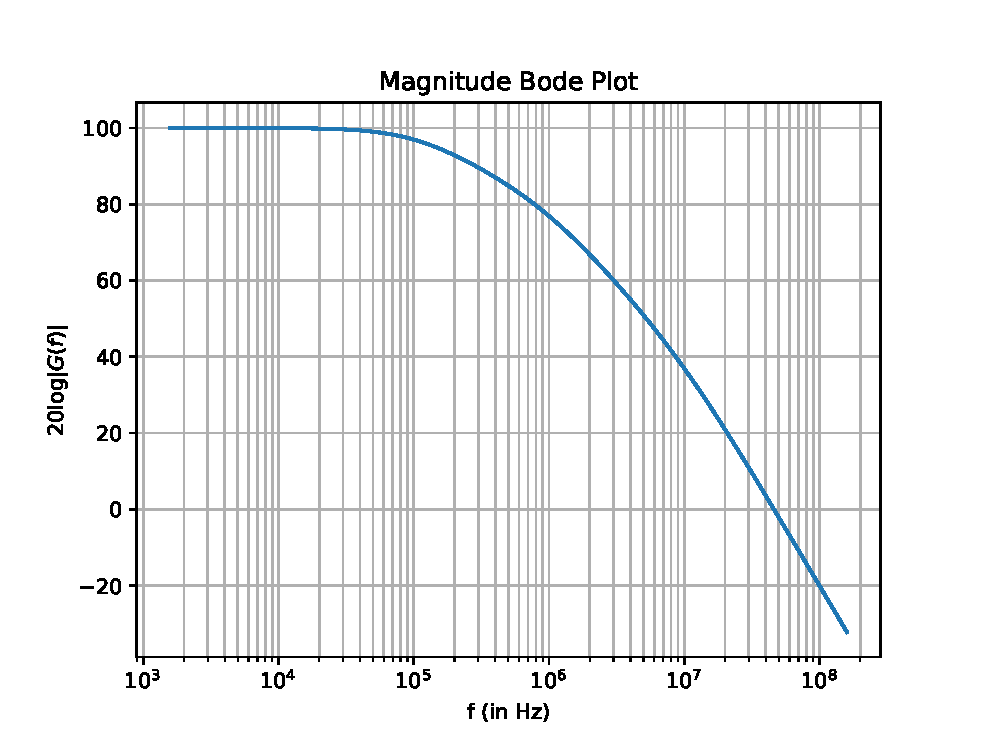
\includegraphics[width=\columnwidth]{./figs/ee18btech11014/Magnitude_Plot.eps}
	\end{center}
	\caption{Magnitude Bode Plot}
	\label{fig:Magnitude Plot}
\end{figure}

Phase Plot is \ref{fig:Phase Plot}
\begin{figure}[ht!]
	\begin{center}
		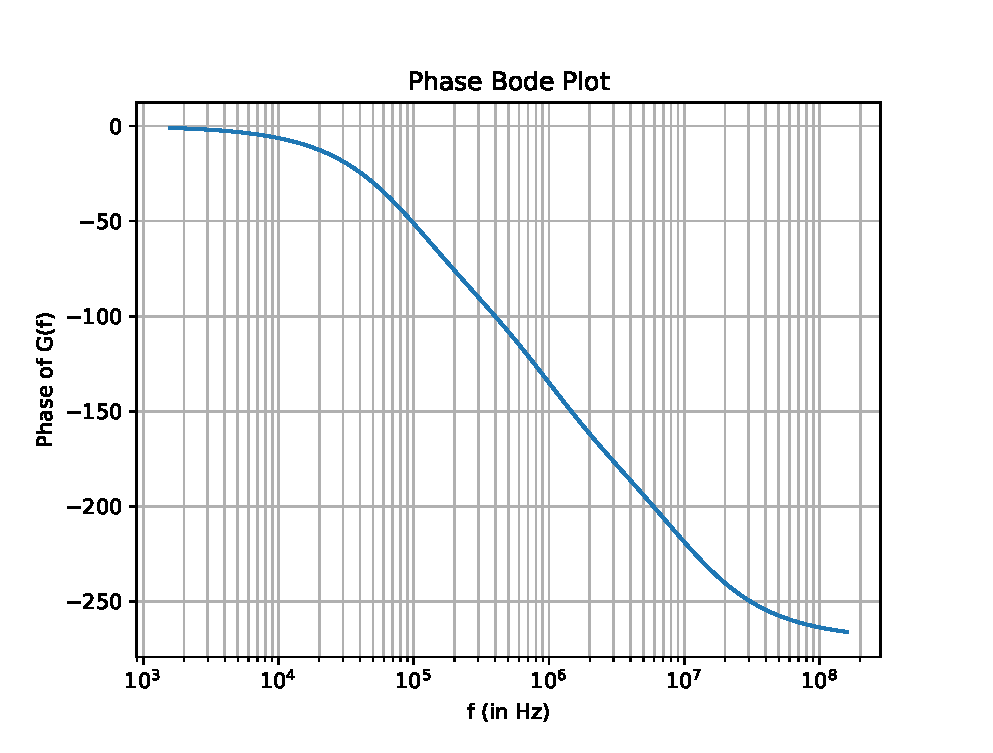
\includegraphics[width=\columnwidth]{./figs/ee18btech11014/Phase_Plot.eps}
	\end{center}
	\caption{Phase Bode Plot}
	\label{fig:Phase Plot}
\end{figure}

Python Code for Magnitude and Phase Bode Plots is at
\begin{lstlisting}
codes/ee18btech11014/Bode_Plot.py
\end{lstlisting}

%-------------------------------------------------------------------------------------------------%
%2.1.13
\item  Design a Closed-Loop Transfer Function by combining both the Open-Loop and Feedback Circuits. Also draw its Equivalent Circuit\\
\solution\\
The Closed-Loop Circuit is
\begin{figure}[ht!]
	\begin{center}
		\resizebox{\columnwidth}{!}{\begin{circuitikz}[american]

\draw (2,2)  node[op amp] (OA) {};
\draw (OA.up) -- ++(0, 0.3) node[vcc]{$+10V$};
\draw (OA.down) -- ++(0,-0.3) node[vee]{$-10V$};
\draw (OA.+) -- (0,1.5) to[vsourcesin, l= $v_{s}$] (0,0) node[ground](GND){};
\draw (OA.-) -- (0,2.5) to[R=$10\ohm$] (-2,2.5) node[ground, rotate=270](GND){};
\draw (OA.out) -- (3,2) node[label={below:$v_{a}$}]{};
\draw (3,2) to[R=$10^{2}\ohm$] (5.5,2) node[label={above:$v_{b}$}]{} to[C,l_=$\frac{10^{-9}}{2\pi}F$] (5.5,0) node[ground](GND){};
\draw (5.5,2) to[R=$10^{3}\ohm$] (8,2) node[label={above:$v_{c}$}]{} to[C,l_=$\frac{10^{-9}}{2\pi}F$] (8,0) node[ground](GND){};
\draw (8,2) to[R=$10^{4}\ohm$] (10.5,2) to[C,l_=$\frac{10^{-9}}{2\pi}F$] (10.5,0) node[ground](GND){};
\draw (10.5,2) -- (11.5,2) node[label={above:$v_{o}$}]{};
\draw (10.5,2) -- (10.5,4) to[R=$1.778\times 10^{5}\ohm$] (0,4) -- (0,2.5);

\end{circuitikz}
}
	\end{center}
	\caption{}
	\label{fig:ee18btech11014_Closed-Loop Circuit}
\end{figure}

The Equivalent Circuit of Closed-Loop Circuit is
\begin{figure}[ht!]
	\begin{center}
		\resizebox{\columnwidth}{!}{\begin{circuitikz}[american]-1
\draw (-3,0) node[ground](GND){} to[vsourcesin, l= $v_{s}$] (-3,2) to[short,-o] (0.25,2) node[label={below:$+$}]{};
\draw (0,0.1) to[R=$10\ohm$,v=$v_{f}$] (-2,0.1) node[ground](GND){}; 
\draw (0,0.1) -- (1,0.1) -- (1,4) to[R=$1.778\times 10^{5}\ohm$] (10.5,4) -- (10.5,2);


\draw (0.25,0.1) to[short,-o] (0.25,0.1) node[label={above:$-$}]{};
\draw (0.25,0.625) node[label={$v_{i}$}] {};


\draw (3,2) node[label={above:$v_{a}$}]{};
\draw (3,0) node[ground](GND){} to[vsourcesin, l= $10^5 v_{i}$] (3,2);
\draw (3,2) to[R=$10^{2}\ohm$] (5.5,2) node[label={above:$v_{b}$}]{} to[C,l_=$\frac{10^{-9}}{2\pi}F$] (5.5,0) node[ground](GND){};
\draw (5.5,2) to[R=$10^{3}\ohm$] (8,2) node[label={above:$v_{c}$}]{} to[C,l_=$\frac{10^{-9}}{2\pi}F$] (8,0) node[ground](GND){};
\draw (8,2) to[R=$10^{4}\ohm$] (10.5,2) to[C,l_=$\frac{10^{-9}}{2\pi}F$] (10.5,0) node[ground](GND){};
\draw (10.5,2) -- (11.5,2) node[label={above:$v_{o}$}]{};

\end{circuitikz}
}
	\end{center},
	\caption{}
	\label{fig:ee18btech11014_Closed-Loop Equivalent Circuit}
\end{figure}

From the Equivalent Circuit Diagram,
\begin{align}
G = \frac{v_{o}}{v_{i}} = \dfrac{10^5}{\left(1+j\frac{f}{10^{5}}\right)\left(1+j\frac{f}{10^{6}}\right)\left(1+j\frac{f}{10^{7}}\right)}\\
H = \frac{v_{f}}{v_{o}} = 5.623 \times 10^{-5}
\end{align}

The Closed-Loop Gain,
\begin{align}
v_{i} = v_{s} - v_{f}\\
\frac{v_{o}}{G} = v_{s} - Hv_{o}\\
\frac{v_{o}}{v_{s}} = \frac{G}{1+GH}
\end{align}

So, the Closed-Loop Gain,
\begin{align}
T = \frac{v_{o}}{v_{s}} = \dfrac{10^5}{5.623 + \left(1+j\frac{f}{10^{5}}\right)\left(1+j\frac{f}{10^{6}}\right)\left(1+j\frac{f}{10^{7}}\right)}
\end{align}

\end{enumerate}

\subsection{Practical Case}
%%\begin{enumerate}[label=\arabic*.,ref=\theenumi]
\begin{enumerate}[label=\thesection.\arabic*.,ref=\thesection.\theenumi]
\numberwithin{equation}{enumi}
%-------------------------------------------------------------------------------------------------%
%2.1.6
\item Find the frequency for which $PM = 90 \degree$.  Assume $H$ to be constant.
\\
%\solution Letting 
%\item Find the frequencies for which phase margins are $90\degree$ and $45\degree$ respectively?\\
\solution $\because \phase{H\brak{f}} = 1$, 
\begin{align}
\phase{G\brak{f_{90}}H\brak{f_{90}}} &= \phase{G\brak{f_{90}}} = 90\degree - 180\degree
\\
&= -90\degree
\label{eq:ee18btech11014_Gpm90}
%\\
%\implies \abs{G\brak{f_{90}}H\brak{f_{90}}} &=1
\end{align}
%
%From \eqref{eq:ee18btech11014_G_ang},
%%
%\begin{multline}
%\phi\brak{f} =
%\\
%-\sbrak{\tan ^{-1}\brak{\frac{f}{10^{5}}}+\tan ^{-1}\brak{\frac{f}{10^{6}}}+\tan ^{-1}\brak{\frac{f}{10^{7}}}}
%\end{multline}
The Bode plot in Fig. 	\ref{fig:ee18btech11014_Bode} shows that 
\begin{align}
\abs{G(f)} < 1, \quad f > 10^8
\end{align}
%
Also, 
\begin{align}
\tan^{-1}\brak{\frac{f}{10^{7}}} \approx 0, \quad f < 10^8
\end{align}

Thus, from  \eqref{eq:ee18btech11014_G_ang} and \eqref{eq:ee18btech11014_Gpm90},
%
\begin{align}
\phi\brak{f} &\approx
-\sbrak{\tan ^{-1}\brak{\frac{f}{10^{5}}}+\tan ^{-1}\brak{\frac{f}{10^{6}}}}
\\
&= -90 \degree
\\
\implies f_{90} &= 3.162 \times 10^{5}
\end{align}
after simplification.
%-------------------------------------------------------------------------------------------------%
\item Find $H$ when the $PM = 90 \degree$.
\\
\solution By definition of the PM, 
\begin{align}
\abs{G\brak{f_{90}}H\brak{f_{90}}} &=1
\\
\implies \abs{H\brak{f_{90}}} &=\frac{1}{\abs{G\brak{f_{90}}}}
\label{eq:ee18btech11014_GH_PM_90}
\end{align}
%
From \eqref{eq:ee18btech11014_G_piece},
\begin{align}
20 \log \abs{G(f)} &= 200 - 20\log(3.162 \times 10^{5})\\
&= 90 dB \\
\implies \abs{G(f)} &= 3.1625 \times 10^{4}
\\
\implies H &= 3.162 \times 10^{-5}
\end{align}
using \eqref{eq:ee18btech11014_GH_PM_90}.
%-------------------------------------------------------------------------------------------------%
\item Design the closed loop circuit for $PM = 90 \degree$
\\
\solution See Fig. 	\ref{fig:ee18btech11014_Closed-Loop Circuit alpha=90}, where Fig. 	\ref{fig:ee18btech11014_Feedback Circuit} is used for the feedback $H$ with $R_M = 0.3162 M \ohm$ and 	$R_F = 10 \ohm$.

\begin{figure}[ht!]
	\begin{center}
		\resizebox{\columnwidth}{!}{\begin{circuitikz}[american]

\draw (2,2)  node[op amp] (OA) {};
\draw (OA.up) -- ++(0, 0.3) node[vcc]{$+10V$};
\draw (OA.down) -- ++(0,-0.3) node[vee]{$-10V$};
\draw (OA.+) -- (0,1.5) to[vsourcesin, l= $v_{s}$] (0,0) node[ground](GND){};
\draw (OA.-) -- (0,2.5) to[R=$10\ohm$] (-2,2.5) node[ground, rotate=270](GND){};
\draw (OA.out) -- (3,2) node[label={below:$v_{a}$}]{};
\draw (3,2) to[R=$10^{2}\ohm$] (5.5,2) node[label={above:$v_{b}$}]{} to[C,l_=$\frac{10^{-9}}{2\pi}F$] (5.5,0) node[ground](GND){};
\draw (5.5,2) to[R=$10^{3}\ohm$] (8,2) node[label={above:$v_{c}$}]{} to[C,l_=$\frac{10^{-9}}{2\pi}F$] (8,0) node[ground](GND){};
\draw (8,2) to[R=$10^{4}\ohm$] (10.5,2) to[C,l_=$\frac{10^{-9}}{2\pi}F$] (10.5,0) node[ground](GND){};
\draw (10.5,2) -- (11.5,2) node[label={above:$v_{o}$}]{};
\draw (10.5,2) -- (10.5,4) to[R=$3.162\times 10^{5}\ohm$] (0,4) -- (0,2.5);

\end{circuitikz}
}
	\end{center}
	\caption{}
	\label{fig:ee18btech11014_Closed-Loop Circuit alpha=90}
\end{figure}

%-------------------------------------------------------------------------------------------------%
\item Repeat all the above for $PM = 45\degree$.
%-------------------------------------------------------------------------------------------------%

%-\tan^{-1}\left(f/10^{5}\right)-\tan^{-1}\left(f/10^{6}\right) = -90\\
%\tan^{-1}\left(f/10^{5}\right)+\tan^{-1}\left(f/10^{6}\right) = 90\\
%\tan^{-1}\left(f/10^{5}\right) = 90-\tan^{-1}\left(f/10^{6}\right)\\
%\tan^{-1}\left(f/10^{5}\right) = \cot^{-1}\left(f/10^{6}\right)\\
%\tan^{-1}\left(f/10^{5}\right) = \tan^{-1}\left(10^{6}/f\right)\\
%f^{2} = 10^{11}\\
%f = 3.162 \times 10^{5}
%\end{align}
%
%So, the approximate value of $f$ at which Phase Margin is $90\degree$ is $f=3.162 \times 10^{5} Hz$.\\

%Similarly let Phase Margin be $\alpha = 45\degree$. Then,
%\begin{align}
%\alpha = \phi - (-180\degree)\\
%\phi = -180\degree + \alpha\\
%\phi = -135\degree
%\end{align}
%
%So, by the definition of Phase-Margin, at $\phi = -135\degree$ , $|GH| = 1 $.  The value of $\phi = -135\degree$ aproximately at poles $f=10^{6} Hz$. 
%
%So, the approximate value of $f$ at which Phase Margin is $45\degree$ is $f=10^{6}$.\\
%%-------------------------------------------------------------------------------------------------%
%%2.1.7
%\item Find the minimum values of Closed-Loop Voltage Gain for which phase margins are $90\degree$ and  $45\degree$ respectively\\
%\solution\\
%For $\alpha=90\degree$,
%\begin{align}
%f=3.162 \times 10^{5}
%\end{align}
%By substituting $f$ in Open-Loop Gain $G(f)$ (assuming poles are far part), 
%\begin{align}
%G(f) = 200 - 20log(3.162 \times 10^{5})\\
%G(f) = 90 dB \\
%G = 3.1625 \times 10^{4}
%\end{align}
%
%At that $f=3.162 \times 10^{5}$, 
%\begin{align}
%H = \frac{1}{G}\\
%H = 3.162 \times 10^{-5}
%\end{align}
%
%The minimum value of Closed-Loop Gain occurs at $|GH| \gg 1$ and the value of Closed-Loop Gain is $T=\frac{1}{H}$
%
%\begin{align}
%T = \frac{1}{H} = 3.1625 \times 10^{4}
%\end{align}
%
%\textbf{So, The minimum value of Closed-Loop Gain with Phase Margin equal to $\alpha=90\degree$ is $T_{min} = 3.1625 \times 10^{4}$.}\\
%
%For $\alpha=45\degree$,
%\begin{align}
%f=10^{6}
%\end{align}
%By substituting $f$ in Open-Loop Gain $G(f)$ (assuming poles are far part), 
%\begin{align}
%G(f) = 200 - 20log(10^{6})\\
%G(f) = 80 dB \\
%G = 10^{4}
%\end{align}
%
%At that $f = 10^{6}$, 
%\begin{align}
%H = \frac{1}{G}\\
%H = 10^{-4}
%\end{align}
%
%The minimum value of Closed-Loop Gain occurs at $|GH| \gg 1$ and the value of Closed-Loop Gain is $T=\frac{1}{H}$
%
%\begin{align}
%T = \frac{1}{H} = 10^{4}
%\end{align}
%
%\textbf{So, The minimum value of Closed-Loop Gain with Phase Margin equal to $\alpha=45\degree$ is $T_{min} = 10^{4}$.}\\
%%-------------------------------------------------------------------------------------------------%
%
%\item Design a Feedback circuit for Phase Margin $\alpha=45^{\circ}$.\\
%\solution
%\begin{figure}[ht!]
%	\begin{center}
%		\resizebox{\columnwidth/2}{!}{\begin{circuitikz}[american]
\ctikzset{tripoles/mos style/arrows}
\draw (1,2) to[short, -o] (0,2) node[label={below:$v_{o}$}]{};
\draw (1,2) to[R=$100k\ohm$] (2,2) -- (3,2) to[R=$10\ohm$] (3,0) node[ground](GND){};
\draw (3,2) to[short, -o] (4,2) node[label={below:$v_{f}$}]{};
\end{circuitikz}
}
%	\end{center},
%	\caption{}
%	\label{fig:ee18btech11014_alpha=45}
%\end{figure}
%\begin{align}
%v_{f} = \frac{10}{10 + 10^{5}} \times v_{o}\\
%v_{f} \approx 10^{-4} v_{o}\\
%\frac{v_{f}}{v_{o}} \approx 10^{-4}\\
%H(s) = 10^{-4}
%\end{align}
%%-------------------------------------------------------------------------------------------------%
%
%\item Design a Feedback circuit for Phase Margin $\alpha=90^{\circ}$.\\
%\solution
%\begin{figure}[ht!]
%	\begin{center}
%		\resizebox{\columnwidth/2}{!}{\begin{circuitikz}[american]
\ctikzset{tripoles/mos style/arrows}
\draw (1,2) to[short, -o] (0,2) node[label={below:$v_{o}$}]{};
\draw (1,2) to[R=$0.3162 M\ohm$] (2,2) -- (3,2) to[R=$10\ohm$] (3,0) node[ground](GND){};
\draw (3,2) to[short, -o] (4,2) node[label={below:$v_{f}$}]{};
\end{circuitikz}
}
%	\end{center},
%	\caption{}
%	\label{fig:ee18btech11014_alpha=90}
%\end{figure}
%\begin{align}
%v_{f} = \frac{10}{10 + 3.162\times 10^{5}} \times v_{o}\\
%v_{f} \approx 3.162\times 10^{-5} v_{o}\\
%\frac{v_{f}}{v_{o}} \approx 3.162\times 10^{-5}\\
%H(s) = 3.162\times 10^{-5}
%\end{align}
%%-------------------------------------------------------------------------------------------------%
%
%\item  Design a Closed-Loop Transfer Function by combining both the Open-Loop and Feedback Circuits for phase Margin $\alpha=45^{\circ}$. Also draw its Equivalent Circuit\\
%\solution\\
%The Closed-Loop Circuit is
%\begin{figure}[ht!]
%	\begin{center}
%		\resizebox{\columnwidth}{!}{\begin{circuitikz}[american]

\draw (2,2)  node[op amp] (OA) {};
\draw (OA.up) -- ++(0, 0.3) node[vcc]{$+10V$};
\draw (OA.down) -- ++(0,-0.3) node[vee]{$-10V$};
\draw (OA.+) -- (0,1.5) to[vsourcesin, l= $v_{s}$] (0,0) node[ground](GND){};
\draw (OA.-) -- (0,2.5) to[R=$10\ohm$] (-2,2.5) node[ground, rotate=270](GND){};
\draw (OA.out) -- (3,2) node[label={below:$v_{a}$}]{};
\draw (3,2) to[R=$10^{2}\ohm$] (5.5,2) node[label={above:$v_{b}$}]{} to[C,l_=$\frac{10^{-9}}{2\pi}F$] (5.5,0) node[ground](GND){};
\draw (5.5,2) to[R=$10^{3}\ohm$] (8,2) node[label={above:$v_{c}$}]{} to[C,l_=$\frac{10^{-9}}{2\pi}F$] (8,0) node[ground](GND){};
\draw (8,2) to[R=$10^{4}\ohm$] (10.5,2) to[C,l_=$\frac{10^{-9}}{2\pi}F$] (10.5,0) node[ground](GND){};
\draw (10.5,2) -- (11.5,2) node[label={above:$v_{o}$}]{};
\draw (10.5,2) -- (10.5,4) to[R=$10^{5}\ohm$] (0,4) -- (0,2.5);

\end{circuitikz}
}
%	\end{center}
%	\caption{}
%	\label{fig:ee18btech11014_Closed-Loop Circuit alpha=45}
%\end{figure}
%
%The Equivalent Circuit of Closed-Loop Circuit is
%\begin{figure}[ht!]
%	\begin{center}
%		\resizebox{\columnwidth}{!}{\begin{circuitikz}[american]-1
\draw (-3,0) node[ground](GND){} to[vsourcesin, l= $v_{s}$] (-3,2) to[short,-o] (0.25,2) node[label={below:$+$}]{};
\draw (0,0.1) to[R=$10\ohm$,v=$v_{f}$] (-2,0.1) node[ground](GND){}; 
\draw (0,0.1) -- (1,0.1) -- (1,4) to[R=$10^{5}\ohm$] (10.5,4) -- (10.5,2);


\draw (0.25,0.1) to[short,-o] (0.25,0.1) node[label={above:$-$}]{};
\draw (0.25,0.625) node[label={$v_{i}$}] {};


\draw (3,2) node[label={above:$v_{a}$}]{};
\draw (3,0) node[ground](GND){} to[vsourcesin, l= $10^5 v_{i}$] (3,2);
\draw (3,2) to[R=$10^{2}\ohm$] (5.5,2) node[label={above:$v_{b}$}]{} to[C,l_=$\frac{10^{-9}}{2\pi}F$] (5.5,0) node[ground](GND){};
\draw (5.5,2) to[R=$10^{3}\ohm$] (8,2) node[label={above:$v_{c}$}]{} to[C,l_=$\frac{10^{-9}}{2\pi}F$] (8,0) node[ground](GND){};
\draw (8,2) to[R=$10^{4}\ohm$] (10.5,2) to[C,l_=$\frac{10^{-9}}{2\pi}F$] (10.5,0) node[ground](GND){};
\draw (10.5,2) -- (11.5,2) node[label={above:$v_{o}$}]{};

\end{circuitikz}
}
%	\end{center},
%	\caption{}
%	\label{fig:ee18btech11014_Closed-Loop Equivalent Circuit alpha=45}
%\end{figure}
%
%From the Equivalent Circuit Diagram,
%\begin{align}
%G(s) = \dfrac{10^5}{\left(1+\frac{s}{2\pi 10^{5}}\right)\left(1+\frac{s}{2\pi 10^{6}}\right)\left(1+\frac{s}{2\pi 10^{7}}\right)}\\
%H(s) = \frac{v_{f}}{v_{o}} = 10^{-4}
%\end{align}
%
%The Closed-Loop Gain,
%\begin{align}
%v_{i} = v_{s} - v_{f}\\
%\frac{v_{o}}{G} = v_{s} - Hv_{o}\\
%\frac{v_{o}}{v_{s}} = \frac{G}{1+GH}
%\end{align}
%
%So, the Closed-Loop Gain,
%\begin{align}
%T(s) = \frac{v_{o}}{v_{s}} = \dfrac{10^5}{10 + \left(1+s\frac{s}{2\pi 10^{5}}\right)\left(1+\frac{s}{2\pi 10^{6}}\right)\left(1+j\frac{s}{2\pi 10^{7}}\right)}
%\end{align}
%%-------------------------------------------------------------------------------------------------%
%
%\item  Design a Closed-Loop Transfer Function by combining both the Open-Loop and Feedback Circuits for phase Margin $\alpha=90^{\circ}$. Also draw its Equivalent Circuit\\
%\solution\\
%The Closed-Loop Circuit is
%\begin{figure}[ht!]
%	\begin{center}
%		\resizebox{\columnwidth}{!}{\begin{circuitikz}[american]

\draw (2,2)  node[op amp] (OA) {};
\draw (OA.up) -- ++(0, 0.3) node[vcc]{$+10V$};
\draw (OA.down) -- ++(0,-0.3) node[vee]{$-10V$};
\draw (OA.+) -- (0,1.5) to[vsourcesin, l= $v_{s}$] (0,0) node[ground](GND){};
\draw (OA.-) -- (0,2.5) to[R=$10\ohm$] (-2,2.5) node[ground, rotate=270](GND){};
\draw (OA.out) -- (3,2) node[label={below:$v_{a}$}]{};
\draw (3,2) to[R=$10^{2}\ohm$] (5.5,2) node[label={above:$v_{b}$}]{} to[C,l_=$\frac{10^{-9}}{2\pi}F$] (5.5,0) node[ground](GND){};
\draw (5.5,2) to[R=$10^{3}\ohm$] (8,2) node[label={above:$v_{c}$}]{} to[C,l_=$\frac{10^{-9}}{2\pi}F$] (8,0) node[ground](GND){};
\draw (8,2) to[R=$10^{4}\ohm$] (10.5,2) to[C,l_=$\frac{10^{-9}}{2\pi}F$] (10.5,0) node[ground](GND){};
\draw (10.5,2) -- (11.5,2) node[label={above:$v_{o}$}]{};
\draw (10.5,2) -- (10.5,4) to[R=$3.162\times 10^{5}\ohm$] (0,4) -- (0,2.5);

\end{circuitikz}
}
%	\end{center}
%	\caption{}
%	\label{fig:ee18btech11014_Closed-Loop Circuit alpha=90}
%\end{figure}
%
%The Equivalent Circuit of Closed-Loop Circuit is
%\begin{figure}[ht!]
%	\begin{center}
%		\resizebox{\columnwidth}{!}{\begin{circuitikz}[american]-1
\draw (-3,0) node[ground](GND){} to[vsourcesin, l= $v_{s}$] (-3,2) to[short,-o] (0.25,2) node[label={below:$+$}]{};
\draw (0,0.1) to[R=$10\ohm$,v=$v_{f}$] (-2,0.1) node[ground](GND){}; 
\draw (0,0.1) -- (1,0.1) -- (1,4) to[R=$3.162\times 10^{5}\ohm$] (10.5,4) -- (10.5,2);


\draw (0.25,0.1) to[short,-o] (0.25,0.1) node[label={above:$-$}]{};
\draw (0.25,0.625) node[label={$v_{i}$}] {};


\draw (3,2) node[label={above:$v_{a}$}]{};
\draw (3,0) node[ground](GND){} to[vsourcesin, l= $10^5 v_{i}$] (3,2);
\draw (3,2) to[R=$10^{2}\ohm$] (5.5,2) node[label={above:$v_{b}$}]{} to[C,l_=$\frac{10^{-9}}{2\pi}F$] (5.5,0) node[ground](GND){};
\draw (5.5,2) to[R=$10^{3}\ohm$] (8,2) node[label={above:$v_{c}$}]{} to[C,l_=$\frac{10^{-9}}{2\pi}F$] (8,0) node[ground](GND){};
\draw (8,2) to[R=$10^{4}\ohm$] (10.5,2) to[C,l_=$\frac{10^{-9}}{2\pi}F$] (10.5,0) node[ground](GND){};
\draw (10.5,2) -- (11.5,2) node[label={above:$v_{o}$}]{};

\end{circuitikz}
}
%	\end{center},
%	\caption{}
%	\label{fig:ee18btech11014_Closed-Loop Equivalent Circuit alpha=90}
%\end{figure}
%
%From the Equivalent Circuit Diagram,
%\begin{align}
%G(s) = \dfrac{10^5}{\left(1+\frac{s}{2\pi 10^{5}}\right)\left(1+\frac{s}{2\pi 10^{6}}\right)\left(1+\frac{s}{2\pi 10^{7}}\right)}\\
%H(s) = \frac{v_{f}}{v_{o}} = 3.162\times 10^{-5}
%\end{align}
%
%The Closed-Loop Gain,
%\begin{align}
%v_{i} = v_{s} - v_{f}\\
%\frac{v_{o}}{G} = v_{s} - Hv_{o}\\
%\frac{v_{o}}{v_{s}} = \frac{G}{1+GH}
%\end{align}
%
%So, the Closed-Loop Gain,
%\begin{align}
%T(s) = \frac{v_{o}}{v_{s}} = \dfrac{10^5}{3.162 + \left(1+s\frac{s}{2\pi 10^{5}}\right)\left(1+\frac{s}{2\pi 10^{6}}\right)\left(1+j\frac{s}{2\pi 10^{7}}\right)}
%\end{align}
\end{enumerate}

%
\section{Feedback Current Amplifier: Example}
%\begin{enumerate}[label=\thesubsection.\arabic*.,ref=\thesubsection.\theenumi]
\numberwithin{equation}{enumi}
\item
Consider a Feedback Current Amplifier formed by cascading an Inverting Opamp $\mu$ with a MOSFET (NMOS).
The output current is the Drain Current of the NMOS.
Assume that Opamp has an input resistance $R_{id}$, an Open Circuit Voltage Gain $\mu$, and an output resistance $r_{o1}$

\begin{figure}[!ht]
	\begin{center}
		\resizebox{\columnwidth}{!}{\ctikzset{tripoles/mos style/arrows}
\usetikzlibrary{arrows.meta,decorations.markings}
\begin{circuitikz}
\ctikzset{bipoles/length=1cm}
\draw
(0, 0) node[op amp] (opamp) {$\mu$}
(1.5,0) node[nmos,](Q){}
(opamp.-) -- (-2,0.35) -- (-2,-2) to[R=$R_2$,i=$I_{f}$]
(1.5,-2) --(Q.S){}
(-2,-2) to[short, i=$I_{i}$] (-2,0.35)
(1.5,-0.2) to[short, i=$I_{0}$] (1.5, -2)
(1.5,-2) to[R=$R_1$] (1.5,-4) node[ground]{}
(opamp.+) -- (-1,-0.35) -- (-1,-0.4) node[ground]{}
(Q.center) node[right]{{$Q$}}
(Q.D) -- (1.5,1)-- (2,1) node[ground]{}
(-2,-2) --(-3,-2) to[R=$R_s$] (-3,-4) node[ground]{}
(-4,-4) node[ground]{}
(-4,-4) to[I=$I_s$] (-4,-2) --(-3,-2)
;\end{circuitikz}}
	\end{center}
\caption{Complete Circuit}
\label{fig:Complete_Circuit}
\end{figure}

\item
Represent the given circuit using a Small Signal Equivalent Model.

\solution
\begin{figure}[!ht]
	\begin{center}
		\resizebox{\columnwidth}{!}{\begin{circuitikz}
\ctikzset{bipoles/length=1cm}
\draw
(-0.5,0) to[short,i=$I_i$,*-*] (0.5,0){}
(0.5,0) -- (0.5,-1) to[R=$R_s$] (0.5,-2) --(0.5,-3) node[ground]{}
(0.5,0) -- (1.5,0) -- (1.5,-1) to[R=$R_{id}$] (1.5,-2) --(1.5,-3) node[ground]{}
(1.5,0) -- (2.5,0) -- (2.5,-0.5) to[R=$R_1$] (2.5,-2) to[R=$R_2$] (2.5,-2.5) --(2.5,-3) node[ground]{}
(2.5,0) -- (3.5,0) node at(3.5,-0.2){$+$}
node at(3.5,-3){$-$}
node at(3.5,-1.25){$V_i$}
(5,0) to[R=$r_{01}$,*-*] (7,0){}
(5,-3) node[ground]{}
(5,-3)--(5,-2) to[V=$\mu V_i$]  (5,-1) -- (5,0){}
node at(7,-0.2) {$+$}
node at(7,-3) {$-$}
node at(7,-2) {$V_{gs}$}
(8.5,0) to[I=$g_{m}V{gs}$] (8.5,-2){}
(8.5,0)--((8.5,1) --(9,1) node[ground]{}
(8.5,0) -- (10,0) to[R=$r_{02}$] (10,-2) -- (8.5,-2){}
(8.5,-2) to[short, i = $I_{o}$] (8.5,-3) -- (8.5,-3.5) to[R=$R_1$] (8.5,-4.5) -- (8.5,-5) node[ground]{}
(8.5,-3) -- (7.5,-3) --(7.5,-3.5) to[R=$R_2$] (7.5,-4.5) -- (7.5,-5) node[ground]{}
;\end{circuitikz}
}
	\end{center}
\caption{Small Signal Model}
\label{fig:Small_Signal_Model}
\end{figure}

\item
Represent the Control System using a block diagram

\solution
\begin{figure}[!ht]
	\begin{center}
			\resizebox{\columnwidth}{!}{\tikzstyle{input} = [coordinate]
\tikzstyle{output} = [coordinate]
\tikzstyle{block} = [draw, rectangle]
\tikzstyle{sum} = [draw, circle]

\begin{tikzpicture}[auto, node distance=2cm,>=latex']
    \node [input, name=input] {$I_s$};
    \node [sum, right of=input] (sum) {};
    \node [block, right of=sum] (controller) {$G$};
    \node [output, right of=controller] (output) {};
    \node [block, below of=controller] (feedback) {$H$};
    \draw [draw,->] (input) -- node {$I_{s}$} (sum);
    \draw [->] (sum) -- node {$I_{i}$} (controller);
    \draw [->] (controller) -- node [name=y] {$I_o$}(output);
    \draw [->] (y) |- (feedback);
    \draw [->] (feedback) -| node[pos=0.95]{$-$}  node [near end] {$I_f$} (sum);
    \draw [->] (feedback) -| node[pos=1.15]{$+$}  node [near end] {} (sum);
\end{tikzpicture}
}
	\end{center}
\caption{Block Diagram}
\label{fig:Block_Diagram}
\end{figure}

\item
Describe the resistances involved in the circuit

\solution
\begin{table}[!ht]
\centering
%%%%%%%%%%%%%%%%%%%%%%%%%%%%%%%%%%%%%%%%%%%%%%%%%%%%%%%%%%%%%%%%%%%%%%
%%                                                                  %%
%%  This is the header of a LaTeX2e file exported from Gnumeric.    %%
%%                                                                  %%
%%  This file can be compiled as it stands or included in another   %%
%%  LaTeX document. The table is based on the longtable package so  %%
%%  the longtable options (headers, footers...) can be set in the   %%
%%  preamble section below (see PRAMBLE).                           %%
%%                                                                  %%
%%  To include the file in another, the following two lines must be %%
%%  in the including file:                                          %%
%%        \def\inputGnumericTable{}                                 %%
%%  at the beginning of the file and:                               %%
%%        \input{name-of-this-file.tex}                             %%
%%  where the table is to be placed. Note also that the including   %%
%%  file must use the following packages for the table to be        %%
%%  rendered correctly:                                             %%
%%    \usepackage[latin1]{inputenc}                                 %%
%%    \usepackage{color}                                            %%
%%    \usepackage{array}                                            %%
%%    \usepackage{longtable}                                        %%
%%    \usepackage{calc}                                             %%
%%    \usepackage{multirow}                                         %%
%%    \usepackage{hhline}                                           %%
%%    \usepackage{ifthen}                                           %%
%%  optionally (for landscape tables embedded in another document): %%
%%    \usepackage{lscape}                                           %%
%%                                                                  %%
%%%%%%%%%%%%%%%%%%%%%%%%%%%%%%%%%%%%%%%%%%%%%%%%%%%%%%%%%%%%%%%%%%%%%%



%%  This section checks if we are begin input into another file or  %%
%%  the file will be compiled alone. First use a macro taken from   %%
%%  the TeXbook ex 7.7 (suggestion of Han-Wen Nienhuys).            %%
\def\ifundefined#1{\expandafter\ifx\csname#1\endcsname\relax}


%%  Check for the \def token for inputed files. If it is not        %%
%%  defined, the file will be processed as a standalone and the     %%
%%  preamble will be used.                                          %%
\ifundefined{inputGnumericTable}

%%  We must be able to close or not the document at the end.        %%
	\def\gnumericTableEnd{\end{document}}


%%%%%%%%%%%%%%%%%%%%%%%%%%%%%%%%%%%%%%%%%%%%%%%%%%%%%%%%%%%%%%%%%%%%%%
%%                                                                  %%
%%  This is the PREAMBLE. Change these values to get the right      %%
%%  paper size and other niceties.                                  %%
%%                                                                  %%
%%%%%%%%%%%%%%%%%%%%%%%%%%%%%%%%%%%%%%%%%%%%%%%%%%%%%%%%%%%%%%%%%%%%%%

	\documentclass[12pt%
			  %,landscape%
                    ]{report}
       \usepackage[latin1]{inputenc}
       \usepackage{fullpage}
       \usepackage{color}
       \usepackage{array}
       \usepackage{longtable}
       \usepackage{calc}
       \usepackage{multirow}
       \usepackage{hhline}
       \usepackage{ifthen}

	\begin{document}


%%  End of the preamble for the standalone. The next section is for %%
%%  documents which are included into other LaTeX2e files.          %%
\else

%%  We are not a stand alone document. For a regular table, we will %%
%%  have no preamble and only define the closing to mean nothing.   %%
    \def\gnumericTableEnd{}

%%  If we want landscape mode in an embedded document, comment out  %%
%%  the line above and uncomment the two below. The table will      %%
%%  begin on a new page and run in landscape mode.                  %%
%       \def\gnumericTableEnd{\end{landscape}}
%       \begin{landscape}


%%  End of the else clause for this file being \input.              %%
\fi

%%%%%%%%%%%%%%%%%%%%%%%%%%%%%%%%%%%%%%%%%%%%%%%%%%%%%%%%%%%%%%%%%%%%%%
%%                                                                  %%
%%  The rest is the gnumeric table, except for the closing          %%
%%  statement. Changes below will alter the table's appearance.     %%
%%                                                                  %%
%%%%%%%%%%%%%%%%%%%%%%%%%%%%%%%%%%%%%%%%%%%%%%%%%%%%%%%%%%%%%%%%%%%%%%

\providecommand{\gnumericmathit}[1]{#1} 
%%  Uncomment the next line if you would like your numbers to be in %%
%%  italics if they are italizised in the gnumeric table.           %%
%\renewcommand{\gnumericmathit}[1]{\mathit{#1}}
\providecommand{\gnumericPB}[1]%
{\let\gnumericTemp=\\#1\let\\=\gnumericTemp\hspace{0pt}}
 \ifundefined{gnumericTableWidthDefined}
        \newlength{\gnumericTableWidth}
        \newlength{\gnumericTableWidthComplete}
        \newlength{\gnumericMultiRowLength}
        \global\def\gnumericTableWidthDefined{}
 \fi
%% The following setting protects this code from babel shorthands.  %%
 \ifthenelse{\isundefined{\languageshorthands}}{}{\languageshorthands{english}}
%%  The default table format retains the relative column widths of  %%
%%  gnumeric. They can easily be changed to c, r or l. In that case %%
%%  you may want to comment out the next line and uncomment the one %%
%%  thereafter                                                      %%
\providecommand\gnumbox{\makebox[0pt]}
%%\providecommand\gnumbox[1][]{\makebox}

%% to adjust positions in multirow situations                       %%
\setlength{\bigstrutjot}{\jot}
\setlength{\extrarowheight}{\doublerulesep}

%%  The \setlongtables command keeps column widths the same across  %%
%%  pages. Simply comment out next line for varying column widths.  %%
\setlongtables

\setlength\gnumericTableWidth{%
	53pt+%
	163pt+%
0pt}
\def\gumericNumCols{2}
\setlength\gnumericTableWidthComplete{\gnumericTableWidth+%
         \tabcolsep*\gumericNumCols*2+\arrayrulewidth*\gumericNumCols}
\ifthenelse{\lengthtest{\gnumericTableWidthComplete > \linewidth}}%
         {\def\gnumericScale{\ratio{\linewidth-%
                        \tabcolsep*\gumericNumCols*2-%
                        \arrayrulewidth*\gumericNumCols}%
{\gnumericTableWidth}}}%
{\def\gnumericScale{1}}

%%%%%%%%%%%%%%%%%%%%%%%%%%%%%%%%%%%%%%%%%%%%%%%%%%%%%%%%%%%%%%%%%%%%%%
%%                                                                  %%
%% The following are the widths of the various columns. We are      %%
%% defining them here because then they are easier to change.       %%
%% Depending on the cell formats we may use them more than once.    %%
%%                                                                  %%
%%%%%%%%%%%%%%%%%%%%%%%%%%%%%%%%%%%%%%%%%%%%%%%%%%%%%%%%%%%%%%%%%%%%%%

\ifthenelse{\isundefined{\gnumericColA}}{\newlength{\gnumericColA}}{}\settowidth{\gnumericColA}{\begin{tabular}{@{}p{53pt*\gnumericScale}@{}}x\end{tabular}}
\ifthenelse{\isundefined{\gnumericColB}}{\newlength{\gnumericColB}}{}\settowidth{\gnumericColB}{\begin{tabular}{@{}p{163pt*\gnumericScale}@{}}x\end{tabular}}

\begin{tabular}[c]{%
	b{\gnumericColA}%
	b{\gnumericColB}%
	}

%%%%%%%%%%%%%%%%%%%%%%%%%%%%%%%%%%%%%%%%%%%%%%%%%%%%%%%%%%%%%%%%%%%%%%
%%  The longtable options. (Caption, headers... see Goosens, p.124) %%
%	\caption{The Table Caption.}             \\	%
% \hline	% Across the top of the table.
%%  The rest of these options are table rows which are placed on    %%
%%  the first, last or every page. Use \multicolumn if you want.    %%

%%  Header for the first page.                                      %%
%	\multicolumn{2}{c}{The First Header} \\ \hline 
%	\multicolumn{1}{c}{colTag}	%Column 1
%	&\multicolumn{1}{c}{colTag}	\\ \hline %Last column
%	\endfirsthead

%%  The running header definition.                                  %%
%	\hline
%	\multicolumn{2}{l}{\ldots\small\slshape continued} \\ \hline
%	\multicolumn{1}{c}{colTag}	%Column 1
%	&\multicolumn{1}{c}{colTag}	\\ \hline %Last column
%	\endhead

%%  The running footer definition.                                  %%
%	\hline
%	\multicolumn{2}{r}{\small\slshape continued\ldots} \\
%	\endfoot

%%  The ending footer definition.                                   %%
%	\multicolumn{2}{c}{That's all folks} \\ \hline 
%	\endlastfoot
%%%%%%%%%%%%%%%%%%%%%%%%%%%%%%%%%%%%%%%%%%%%%%%%%%%%%%%%%%%%%%%%%%%%%%

\hhline{|-|-}
	 \multicolumn{1}{|p{\gnumericColA}|}%
	{\gnumericPB{\centering}\gnumbox{\textbf{Resistance}}}
	&\multicolumn{1}{p{\gnumericColB}|}%
	{\gnumericPB{\centering}\gnumbox{\textbf{Description}}}
\\
\hhline{|--|}
	 \multicolumn{1}{|p{\gnumericColA}|}%
	{\gnumericPB{\raggedright}\gnumbox[l]{$R_{i}$}}
	&\multicolumn{1}{p{\gnumericColB}|}%
	{\gnumericPB{\raggedright}\gnumbox[l]{Total Input Resistance}}
\\
\hhline{|--|}
	 \multicolumn{1}{|p{\gnumericColA}|}%
	{\gnumericPB{\raggedright}\gnumbox[l]{$R_{out}$}}
	&\multicolumn{1}{p{\gnumericColB}|}%
	{\gnumericPB{\raggedright}\gnumbox[l]{Total Ouput Resistance}}
\\
\hhline{|--|}
	 \multicolumn{1}{|p{\gnumericColA}|}%
	{\gnumericPB{\raggedright}\gnumbox[l]{$R_{id}$}}
	&\multicolumn{1}{p{\gnumericColB}|}%
	{\gnumericPB{\raggedright}\gnumbox[l]{Input resistance of Opamp}}
\\
\hhline{|--|}
	 \multicolumn{1}{|p{\gnumericColA}|}%
	{\gnumericPB{\raggedright}\gnumbox[l]{$r_{o1}$}}
	&\multicolumn{1}{p{\gnumericColB}|}%
	{\gnumericPB{\raggedright}\gnumbox[l]{Output resistance of Opamp}}
\\
\hhline{|--|}
	 \multicolumn{1}{|p{\gnumericColA}|}%
	{\gnumericPB{\raggedright}\gnumbox[l]{$r_{o2}$}}
	&\multicolumn{1}{p{\gnumericColB}|}%
	{\gnumericPB{\raggedright}\gnumbox[l]{Output resistance of MOSFET}}
\\
\hhline{|--|}
	 \multicolumn{1}{|p{\gnumericColA}|}%
	{\gnumericPB{\raggedright}\gnumbox[l]{$R_{i}$}}
	&\multicolumn{1}{p{\gnumericColB}|}%
	{\gnumericPB{\raggedright}\gnumbox[l]{Input resistance of Open Loop}}
\\
\hhline{|--|}
	 \multicolumn{1}{|p{\gnumericColA}|}%
	{\gnumericPB{\raggedright}\gnumbox[l]{$R_{o}$}}
	&\multicolumn{1}{p{\gnumericColB}|}%
	{\gnumericPB{\raggedright}\gnumbox[l]{Output resistance of Open Loop}}
\\
\hhline{|--|}
	 \multicolumn{1}{|p{\gnumericColA}|}%
	{\gnumericPB{\raggedright}\gnumbox[l]{$R_{if}$}}
	&\multicolumn{1}{p{\gnumericColB}|}%
	{\gnumericPB{\raggedright}\gnumbox[l]{Input resistance of Feedback}}
\\
\hhline{|--|}
	 \multicolumn{1}{|p{\gnumericColA}|}%
	{\gnumericPB{\raggedright}\gnumbox[l]{$R_{of}$}}
	&\multicolumn{1}{p{\gnumericColB}|}%
	{\gnumericPB{\raggedright}\gnumbox[l]{Output resistance of Feedback}}
\\
\hhline{|--|}
	 \multicolumn{1}{|p{\gnumericColA}|}%
	{\gnumericPB{\raggedright}\gnumbox[l]{$R_{s}$}}
	&\multicolumn{1}{p{\gnumericColB}|}%
	{\gnumericPB{\raggedright}\gnumbox[l]{Resistance of Current Source}}
\\
\hhline{|-|-|}
\end{tabular}

\ifthenelse{\isundefined{\languageshorthands}}{}{\languageshorthands{\languagename}}
\gnumericTableEnd
\caption{}
\label{table: Resistance_Table}
\end{table}

\item
Find approximate expressions for G, $R_{i}$, $R_{o}$

\solution
\begin{align}
    R_{i}=R_{s}\|R_{i d}\|(R_{1}+R_{2})
\end{align}
\begin{align}
    V_{i}=I_{i} R_{i}
\end{align}
\begin{align}
    I_{o}=-\mu V_{i} \frac{1}{1 / g_{m}+(R_{1}\|R_{2}\| r_{o 2})} \frac{r_{o 2}}{r_{o 2}+(R_{1} \| R_{2})}
\end{align}
\begin{align}
    G = \frac{I_{o}}{I_{i}}=-\mu \frac{R_{i}}{1 / g_{m}+(R_{1}\|R_{2}\| r_{o 2})} \frac{r_{o 2}}{r_{o 2}+(R_{1} \| R_{2})}
\end{align}
We use the approximation
\begin{align}
    1 / g_{m} \ll (R_{1}\|R_{2}\| r_{o 2})
\end{align}
This is because the $\frac{1}{g_{m}}$ is in order of few \ohm s but, $R_{1}$, $R_{2}$ and $r_{o2}$ are in order of k\ohm s 

\begin{align}
    G =-\mu \frac{R_{i}}{R_{1} \| R_{2}}
\end{align}
\begin{align}
    R_{o}=r_{o 2}+(R_{1} \| R_{2})+(g_{m} r_{o 2})(R_{1} \| R_{2})
\end{align}
\begin{align}
    \implies R_{o} \simeq g_{m} r_{o 2}\left(R_{1} \| R_{2}\right)
\end{align}

\item
Find expression for Loop Gain H

\solution
\begin{align}
    H = \frac{I_{f}}{I_{o}}=-\frac{R_{1}}{R_{1}+R_{2}}
\end{align}

\item
If loop gain is large, find approximate expression for closed loop gain $T$

\solution
Given,
\begin{align}
    GH \gg 1
\end{align}
\begin{align}
    T = \frac{G}{1+GH}\simeq \frac{1}{H}
\end{align}


\begin{align}
    T \simeq \frac{1}{H}=-\left(1+\frac{R_{2}}{R_{1}}\right)
\end{align}

\item
Give expressions for GH, $T$, $R_{if}$, $R_{in}$, $R_{of}$, $R_{out}$

\solution
\begin{align}
    GH=\mu \frac{R_{i}}{\frac{1}{g_{m}}+(R_{1}\|R_{2}\| r_{o 2})} \frac{r_{o 2}}{r_{o 2}+(R_{1} \| R_{2})} \frac{R_{1}}{R_{1}+R_{2}}
\end{align}

Once again, using the approximation,
\begin{align}
    \implies GH \simeq \mu \frac{R_{i}}{R_{1} \| R_{2}} \frac{R_{1}}{R_{1}+R_{2}}=\mu \frac{R_{i}}{R_{2}}
\end{align}

For Input Resistance,
\begin{align}
    R_{if}=R_{i} /(1+GH)
\end{align}
\begin{align}
    \implies \frac{1}{R_{i f}}=\frac{1}{R_{i}}+\frac{\mu}{R_{2}}
\end{align}
\begin{align}
    \implies R_{i f}=R_{i} \| \frac{R_{2}}{\mu}
\end{align}

Substituting the value of $R_{i}$,
\begin{align}
    R_{if}=R_{s}\|R_{id}\|(R_{1}+R_{2}) \| \frac{R_{2}}{\mu}
\end{align}

\begin{align}
    R_{if}=R_{s} \| R_{in}
\end{align}

\begin{align}
    \implies R_{in}=R_{i d}\|(R_{1}+R_{2})\| \frac{R_{2}}{\mu}
\end{align}
\begin{align}
    R_{in} \simeq \frac{R_{2}}{\mu}
\end{align}

For Output Resistance,
\begin{align}
    R_{of}=R_{o}(1+GH) \simeq GH R_{o}
\end{align}
\begin{align}
    R_{of} \simeq \mu (\frac{R_{i}}{R_{2}})(g_{m} r_{o 2})(R_{1} \| R_{2})
\end{align}
\begin{align}
    R_{out} = R_{of}=\mu \frac{R_{i}}{R_{1}+R_{2}}(g_{m} r_{o 2}) R_{1}
\end{align}


\item
Given the following values
\begin{table}[!ht]
\centering
%%%%%%%%%%%%%%%%%%%%%%%%%%%%%%%%%%%%%%%%%%%%%%%%%%%%%%%%%%%%%%%%%%%%%%
%%                                                                  %%
%%  This is the header of a LaTeX2e file exported from Gnumeric.    %%
%%                                                                  %%
%%  This file can be compiled as it stands or included in another   %%
%%  LaTeX document. The table is based on the longtable package so  %%
%%  the longtable options (headers, footers...) can be set in the   %%
%%  preamble section below (see PRAMBLE).                           %%
%%                                                                  %%
%%  To include the file in another, the following two lines must be %%
%%  in the including file:                                          %%
%%        \def\inputGnumericTable{}                                 %%
%%  at the beginning of the file and:                               %%
%%        \input{name-of-this-file.tex}                             %%
%%  where the table is to be placed. Note also that the including   %%
%%  file must use the following packages for the table to be        %%
%%  rendered correctly:                                             %%
%%    \usepackage[latin1]{inputenc}                                 %%
%%    \usepackage{color}                                            %%
%%    \usepackage{array}                                            %%
%%    \usepackage{longtable}                                        %%
%%    \usepackage{calc}                                             %%
%%    \usepackage{multirow}                                         %%
%%    \usepackage{hhline}                                           %%
%%    \usepackage{ifthen}                                           %%
%%  optionally (for landscape tables embedded in another document): %%
%%    \usepackage{lscape}                                           %%
%%                                                                  %%
%%%%%%%%%%%%%%%%%%%%%%%%%%%%%%%%%%%%%%%%%%%%%%%%%%%%%%%%%%%%%%%%%%%%%%



%%  This section checks if we are begin input into another file or  %%
%%  the file will be compiled alone. First use a macro taken from   %%
%%  the TeXbook ex 7.7 (suggestion of Han-Wen Nienhuys).            %%
\def\ifundefined#1{\expandafter\ifx\csname#1\endcsname\relax}


%%  Check for the \def token for inputed files. If it is not        %%
%%  defined, the file will be processed as a standalone and the     %%
%%  preamble will be used.                                          %%
\ifundefined{inputGnumericTable}

%%  We must be able to close or not the document at the end.        %%
	\def\gnumericTableEnd{\end{document}}


%%%%%%%%%%%%%%%%%%%%%%%%%%%%%%%%%%%%%%%%%%%%%%%%%%%%%%%%%%%%%%%%%%%%%%
%%                                                                  %%
%%  This is the PREAMBLE. Change these values to get the right      %%
%%  paper size and other niceties.                                  %%
%%                                                                  %%
%%%%%%%%%%%%%%%%%%%%%%%%%%%%%%%%%%%%%%%%%%%%%%%%%%%%%%%%%%%%%%%%%%%%%%

	\documentclass[12pt%
			  %,landscape%
                    ]{report}
       \usepackage[latin1]{inputenc}
       \usepackage{fullpage}
       \usepackage{color}
       \usepackage{array}
       \usepackage{longtable}
       \usepackage{calc}
       \usepackage{multirow}
       \usepackage{hhline}
       \usepackage{ifthen}

	\begin{document}


%%  End of the preamble for the standalone. The next section is for %%
%%  documents which are included into other LaTeX2e files.          %%
\else

%%  We are not a stand alone document. For a regular table, we will %%
%%  have no preamble and only define the closing to mean nothing.   %%
    \def\gnumericTableEnd{}

%%  If we want landscape mode in an embedded document, comment out  %%
%%  the line above and uncomment the two below. The table will      %%
%%  begin on a new page and run in landscape mode.                  %%
%       \def\gnumericTableEnd{\end{landscape}}
%       \begin{landscape}


%%  End of the else clause for this file being \input.              %%
\fi

%%%%%%%%%%%%%%%%%%%%%%%%%%%%%%%%%%%%%%%%%%%%%%%%%%%%%%%%%%%%%%%%%%%%%%
%%                                                                  %%
%%  The rest is the gnumeric table, except for the closing          %%
%%  statement. Changes below will alter the table's appearance.     %%
%%                                                                  %%
%%%%%%%%%%%%%%%%%%%%%%%%%%%%%%%%%%%%%%%%%%%%%%%%%%%%%%%%%%%%%%%%%%%%%%

\providecommand{\gnumericmathit}[1]{#1} 
%%  Uncomment the next line if you would like your numbers to be in %%
%%  italics if they are italizised in the gnumeric table.           %%
%\renewcommand{\gnumericmathit}[1]{\mathit{#1}}
\providecommand{\gnumericPB}[1]%
{\let\gnumericTemp=\\#1\let\\=\gnumericTemp\hspace{0pt}}
 \ifundefined{gnumericTableWidthDefined}
        \newlength{\gnumericTableWidth}
        \newlength{\gnumericTableWidthComplete}
        \newlength{\gnumericMultiRowLength}
        \global\def\gnumericTableWidthDefined{}
 \fi
%% The following setting protects this code from babel shorthands.  %%
 \ifthenelse{\isundefined{\languageshorthands}}{}{\languageshorthands{english}}
%%  The default table format retains the relative column widths of  %%
%%  gnumeric. They can easily be changed to c, r or l. In that case %%
%%  you may want to comment out the next line and uncomment the one %%
%%  thereafter                                                      %%
\providecommand\gnumbox{\makebox[0pt]}
%%\providecommand\gnumbox[1][]{\makebox}

%% to adjust positions in multirow situations                       %%
\setlength{\bigstrutjot}{\jot}
\setlength{\extrarowheight}{\doublerulesep}

%%  The \setlongtables command keeps column widths the same across  %%
%%  pages. Simply comment out next line for varying column widths.  %%
\setlongtables

\setlength\gnumericTableWidth{%
	53pt+%
	93pt+%
0pt}
\def\gumericNumCols{2}
\setlength\gnumericTableWidthComplete{\gnumericTableWidth+%
         \tabcolsep*\gumericNumCols*2+\arrayrulewidth*\gumericNumCols}
\ifthenelse{\lengthtest{\gnumericTableWidthComplete > \linewidth}}%
         {\def\gnumericScale{\ratio{\linewidth-%
                        \tabcolsep*\gumericNumCols*2-%
                        \arrayrulewidth*\gumericNumCols}%
{\gnumericTableWidth}}}%
{\def\gnumericScale{1}}

%%%%%%%%%%%%%%%%%%%%%%%%%%%%%%%%%%%%%%%%%%%%%%%%%%%%%%%%%%%%%%%%%%%%%%
%%                                                                  %%
%% The following are the widths of the various columns. We are      %%
%% defining them here because then they are easier to change.       %%
%% Depending on the cell formats we may use them more than once.    %%
%%                                                                  %%
%%%%%%%%%%%%%%%%%%%%%%%%%%%%%%%%%%%%%%%%%%%%%%%%%%%%%%%%%%%%%%%%%%%%%%

\ifthenelse{\isundefined{\gnumericColA}}{\newlength{\gnumericColA}}{}\settowidth{\gnumericColA}{\begin{tabular}{@{}p{53pt*\gnumericScale}@{}}x\end{tabular}}
\ifthenelse{\isundefined{\gnumericColB}}{\newlength{\gnumericColB}}{}\settowidth{\gnumericColB}{\begin{tabular}{@{}p{93pt*\gnumericScale}@{}}x\end{tabular}}

\begin{tabular}[c]{%
	b{\gnumericColA}%
	b{\gnumericColB}%
	}

%%%%%%%%%%%%%%%%%%%%%%%%%%%%%%%%%%%%%%%%%%%%%%%%%%%%%%%%%%%%%%%%%%%%%%
%%  The longtable options. (Caption, headers... see Goosens, p.124) %%
%	\caption{The Table Caption.}             \\	%
% \hline	% Across the top of the table.
%%  The rest of these options are table rows which are placed on    %%
%%  the first, last or every page. Use \multicolumn if you want.    %%

%%  Header for the first page.                                      %%
%	\multicolumn{2}{c}{The First Header} \\ \hline 
%	\multicolumn{1}{c}{colTag}	%Column 1
%	&\multicolumn{1}{c}{colTag}	\\ \hline %Last column
%	\endfirsthead

%%  The running header definition.                                  %%
%	\hline
%	\multicolumn{2}{l}{\ldots\small\slshape continued} \\ \hline
%	\multicolumn{1}{c}{colTag}	%Column 1
%	&\multicolumn{1}{c}{colTag}	\\ \hline %Last column
%	\endhead

%%  The running footer definition.                                  %%
%	\hline
%	\multicolumn{2}{r}{\small\slshape continued\ldots} \\
%	\endfoot

%%  The ending footer definition.                                   %%
%	\multicolumn{2}{c}{That's all folks} \\ \hline 
%	\endlastfoot
%%%%%%%%%%%%%%%%%%%%%%%%%%%%%%%%%%%%%%%%%%%%%%%%%%%%%%%%%%%%%%%%%%%%%%

\hhline{|-|-}
	 \multicolumn{1}{|p{\gnumericColA}|}%
	{\gnumericPB{\centering}\gnumbox{\textbf{Parameter}}}
	&\multicolumn{1}{p{\gnumericColB}|}%
	{\gnumericPB{\centering}\gnumbox{\textbf{Value}}}
\\
\hhline{|--|}
	 \multicolumn{1}{|p{\gnumericColA}|}%
	{\gnumericPB{\raggedright}\gnumbox[l]{$\mu$}}
	&\multicolumn{1}{p{\gnumericColB}|}%
	{\gnumericPB{\raggedright}\gnumbox[l]{$1000$}}
\\
\hhline{|--|}
	 \multicolumn{1}{|p{\gnumericColA}|}%
	{\gnumericPB{\raggedright}\gnumbox[l]{$R_{s}$}}
	&\multicolumn{1}{p{\gnumericColB}|}%
	{\gnumericPB{\raggedright}\gnumbox[l]{$\infty$}}
\\
\hhline{|--|}
	 \multicolumn{1}{|p{\gnumericColA}|}%
	{\gnumericPB{\raggedright}\gnumbox[l]{$R_{id}$}}
	&\multicolumn{1}{p{\gnumericColB}|}%
	{\gnumericPB{\raggedright}\gnumbox[l]{$\infty$}}
\\
\hhline{|--|}
	 \multicolumn{1}{|p{\gnumericColA}|}%
	{\gnumericPB{\raggedright}\gnumbox[l]{$r_{o1}$}}
	&\multicolumn{1}{p{\gnumericColB}|}%
	{\gnumericPB{\raggedright}\gnumbox[l]{$1k\Omega$}}
\\
\hhline{|--|}
	 \multicolumn{1}{|p{\gnumericColA}|}%
	{\gnumericPB{\raggedright}\gnumbox[l]{$R_{1}$}}
	&\multicolumn{1}{p{\gnumericColB}|}%
	{\gnumericPB{\raggedright}\gnumbox[l]{$10k\Omega$}}
\\
\hhline{|--|}
	 \multicolumn{1}{|p{\gnumericColA}|}%
	{\gnumericPB{\raggedright}\gnumbox[l]{$R_{2}$}}
	&\multicolumn{1}{p{\gnumericColB}|}%
	{\gnumericPB{\raggedright}\gnumbox[l]{$90k\Omega$}}
\\
\hhline{|--|}
	 \multicolumn{1}{|p{\gnumericColA}|}%
	{\gnumericPB{\raggedright}\gnumbox[l]{$g_{m}$}}
	&\multicolumn{1}{p{\gnumericColB}|}%
	{\gnumericPB{\raggedright}\gnumbox[l]{$5mA/V$}}
\\
\hhline{|--|}
	 \multicolumn{1}{|p{\gnumericColA}|}%
	{\gnumericPB{\raggedright}\gnumbox[l]{$r_{o2}$}}
	&\multicolumn{1}{p{\gnumericColB}|}%
	{\gnumericPB{\raggedright}\gnumbox[l]{$20k\Omega$}}
\\
\hhline{|-|-|}
\end{tabular}

\ifthenelse{\isundefined{\languageshorthands}}{}{\languageshorthands{\languagename}}
\gnumericTableEnd

\caption{}
\label{table: Input_Table}
\end{table}

Find numerical value of $R_{i}$ and use it to find the value of G

\solution
Using the given numerical values on the previously obtained equations, we obtain:
\begin{align}
    R_{i}=\infty\|\infty\|(10+90)=100 k\ohm
\end{align}

\begin{align}
    G =-1000 \frac{100}{10 \| 90}=-11.11 \times 10^{3}
\end{align}

\item 
Check the validity of the approximation that we use to neglect $1/g_{m}$

\solution
\begin{align}
    1 / g_{m}=0.2 k\ohm \ll (10\|90\| 20)k\ohm = 6.2k\ohm
\end{align}
Hence, we can see that our approximation is valid

\item
Find the value of feedback gain H and open loop gain GH

\solution
\begin{align}
    H=-\frac{R_{1}}{R_{1}+R_{2}}=-\frac{10}{10+90}=-0.1
\end{align}

\begin{align}
    GH=1111 \gg 1
\end{align}

\item
Find the approximate value of closed loop gain T

\solution
\begin{align}
    T \simeq \frac{1}{H} = -\frac{1}{0.1} = -10
\end{align}

\item
Find the values of $R_{in}$ and $R_{out}$

\solution
\begin{align}
    R_{in}=\frac{R_{2}}{\mu}=\frac{90k\ohm}{1000}=90\ohm
\end{align}
\begin{align}
    R_{o} &=g_{m} r_{o 2}(R_{1} \| R_{2}) =5 \times 20(10 \| 90)=900k\ohm
\end{align}
\begin{align}
    R_{out}=(1+GH) R_{o}=1112 \times 900 \simeq 1000M\ohm
\end{align}

\begin{table}[!ht]
\centering
%%%%%%%%%%%%%%%%%%%%%%%%%%%%%%%%%%%%%%%%%%%%%%%%%%%%%%%%%%%%%%%%%%%%%%
%%                                                                  %%
%%  This is the header of a LaTeX2e file exported from Gnumeric.    %%
%%                                                                  %%
%%  This file can be compiled as it stands or included in another   %%
%%  LaTeX document. The table is based on the longtable package so  %%
%%  the longtable options (headers, footers...) can be set in the   %%
%%  preamble section below (see PRAMBLE).                           %%
%%                                                                  %%
%%  To include the file in another, the following two lines must be %%
%%  in the including file:                                          %%
%%        \def\inputGnumericTable{}                                 %%
%%  at the beginning of the file and:                               %%
%%        \input{name-of-this-file.tex}                             %%
%%  where the table is to be placed. Note also that the including   %%
%%  file must use the following packages for the table to be        %%
%%  rendered correctly:                                             %%
%%    \usepackage[latin1]{inputenc}                                 %%
%%    \usepackage{color}                                            %%
%%    \usepackage{array}                                            %%
%%    \usepackage{longtable}                                        %%
%%    \usepackage{calc}                                             %%
%%    \usepackage{multirow}                                         %%
%%    \usepackage{hhline}                                           %%
%%    \usepackage{ifthen}                                           %%
%%  optionally (for landscape tables embedded in another document): %%
%%    \usepackage{lscape}                                           %%
%%                                                                  %%
%%%%%%%%%%%%%%%%%%%%%%%%%%%%%%%%%%%%%%%%%%%%%%%%%%%%%%%%%%%%%%%%%%%%%%



%%  This section checks if we are begin input into another file or  %%
%%  the file will be compiled alone. First use a macro taken from   %%
%%  the TeXbook ex 7.7 (suggestion of Han-Wen Nienhuys).            %%
\def\ifundefined#1{\expandafter\ifx\csname#1\endcsname\relax}


%%  Check for the \def token for inputed files. If it is not        %%
%%  defined, the file will be processed as a standalone and the     %%
%%  preamble will be used.                                          %%
\ifundefined{inputGnumericTable}

%%  We must be able to close or not the document at the end.        %%
	\def\gnumericTableEnd{\end{document}}


%%%%%%%%%%%%%%%%%%%%%%%%%%%%%%%%%%%%%%%%%%%%%%%%%%%%%%%%%%%%%%%%%%%%%%
%%                                                                  %%
%%  This is the PREAMBLE. Change these values to get the right      %%
%%  paper size and other niceties.                                  %%
%%                                                                  %%
%%%%%%%%%%%%%%%%%%%%%%%%%%%%%%%%%%%%%%%%%%%%%%%%%%%%%%%%%%%%%%%%%%%%%%

	\documentclass[12pt%
			  %,landscape%
                    ]{report}
       \usepackage[latin1]{inputenc}
       \usepackage{fullpage}
       \usepackage{color}
       \usepackage{array}
       \usepackage{longtable}
       \usepackage{calc}
       \usepackage{multirow}
       \usepackage{hhline}
       \usepackage{ifthen}

	\begin{document}


%%  End of the preamble for the standalone. The next section is for %%
%%  documents which are included into other LaTeX2e files.          %%
\else

%%  We are not a stand alone document. For a regular table, we will %%
%%  have no preamble and only define the closing to mean nothing.   %%
    \def\gnumericTableEnd{}

%%  If we want landscape mode in an embedded document, comment out  %%
%%  the line above and uncomment the two below. The table will      %%
%%  begin on a new page and run in landscape mode.                  %%
%       \def\gnumericTableEnd{\end{landscape}}
%       \begin{landscape}


%%  End of the else clause for this file being \input.              %%
\fi

%%%%%%%%%%%%%%%%%%%%%%%%%%%%%%%%%%%%%%%%%%%%%%%%%%%%%%%%%%%%%%%%%%%%%%
%%                                                                  %%
%%  The rest is the gnumeric table, except for the closing          %%
%%  statement. Changes below will alter the table's appearance.     %%
%%                                                                  %%
%%%%%%%%%%%%%%%%%%%%%%%%%%%%%%%%%%%%%%%%%%%%%%%%%%%%%%%%%%%%%%%%%%%%%%

\providecommand{\gnumericmathit}[1]{#1} 
%%  Uncomment the next line if you would like your numbers to be in %%
%%  italics if they are italizised in the gnumeric table.           %%
%\renewcommand{\gnumericmathit}[1]{\mathit{#1}}
\providecommand{\gnumericPB}[1]%
{\let\gnumericTemp=\\#1\let\\=\gnumericTemp\hspace{0pt}}
 \ifundefined{gnumericTableWidthDefined}
        \newlength{\gnumericTableWidth}
        \newlength{\gnumericTableWidthComplete}
        \newlength{\gnumericMultiRowLength}
        \global\def\gnumericTableWidthDefined{}
 \fi
%% The following setting protects this code from babel shorthands.  %%
 \ifthenelse{\isundefined{\languageshorthands}}{}{\languageshorthands{english}}
%%  The default table format retains the relative column widths of  %%
%%  gnumeric. They can easily be changed to c, r or l. In that case %%
%%  you may want to comment out the next line and uncomment the one %%
%%  thereafter                                                      %%
\providecommand\gnumbox{\makebox[0pt]}
%%\providecommand\gnumbox[1][]{\makebox}

%% to adjust positions in multirow situations                       %%
\setlength{\bigstrutjot}{\jot}
\setlength{\extrarowheight}{\doublerulesep}

%%  The \setlongtables command keeps column widths the same across  %%
%%  pages. Simply comment out next line for varying column widths.  %%
\setlongtables

\setlength\gnumericTableWidth{%
	53pt+%
	93pt+%
0pt}
\def\gumericNumCols{2}
\setlength\gnumericTableWidthComplete{\gnumericTableWidth+%
         \tabcolsep*\gumericNumCols*2+\arrayrulewidth*\gumericNumCols}
\ifthenelse{\lengthtest{\gnumericTableWidthComplete > \linewidth}}%
         {\def\gnumericScale{\ratio{\linewidth-%
                        \tabcolsep*\gumericNumCols*2-%
                        \arrayrulewidth*\gumericNumCols}%
{\gnumericTableWidth}}}%
{\def\gnumericScale{1}}

%%%%%%%%%%%%%%%%%%%%%%%%%%%%%%%%%%%%%%%%%%%%%%%%%%%%%%%%%%%%%%%%%%%%%%
%%                                                                  %%
%% The following are the widths of the various columns. We are      %%
%% defining them here because then they are easier to change.       %%
%% Depending on the cell formats we may use them more than once.    %%
%%                                                                  %%
%%%%%%%%%%%%%%%%%%%%%%%%%%%%%%%%%%%%%%%%%%%%%%%%%%%%%%%%%%%%%%%%%%%%%%

\ifthenelse{\isundefined{\gnumericColA}}{\newlength{\gnumericColA}}{}\settowidth{\gnumericColA}{\begin{tabular}{@{}p{53pt*\gnumericScale}@{}}x\end{tabular}}
\ifthenelse{\isundefined{\gnumericColB}}{\newlength{\gnumericColB}}{}\settowidth{\gnumericColB}{\begin{tabular}{@{}p{93pt*\gnumericScale}@{}}x\end{tabular}}

\begin{tabular}[c]{%
	b{\gnumericColA}%
	b{\gnumericColB}%
	}

%%%%%%%%%%%%%%%%%%%%%%%%%%%%%%%%%%%%%%%%%%%%%%%%%%%%%%%%%%%%%%%%%%%%%%
%%  The longtable options. (Caption, headers... see Goosens, p.124) %%
%	\caption{The Table Caption.}             \\	%
% \hline	% Across the top of the table.
%%  The rest of these options are table rows which are placed on    %%
%%  the first, last or every page. Use \multicolumn if you want.    %%

%%  Header for the first page.                                      %%
%	\multicolumn{2}{c}{The First Header} \\ \hline 
%	\multicolumn{1}{c}{colTag}	%Column 1
%	&\multicolumn{1}{c}{colTag}	\\ \hline %Last column
%	\endfirsthead

%%  The running header definition.                                  %%
%	\hline
%	\multicolumn{2}{l}{\ldots\small\slshape continued} \\ \hline
%	\multicolumn{1}{c}{colTag}	%Column 1
%	&\multicolumn{1}{c}{colTag}	\\ \hline %Last column
%	\endhead

%%  The running footer definition.                                  %%
%	\hline
%	\multicolumn{2}{r}{\small\slshape continued\ldots} \\
%	\endfoot

%%  The ending footer definition.                                   %%
%	\multicolumn{2}{c}{That's all folks} \\ \hline 
%	\endlastfoot
%%%%%%%%%%%%%%%%%%%%%%%%%%%%%%%%%%%%%%%%%%%%%%%%%%%%%%%%%%%%%%%%%%%%%%

\hhline{|-|-}
	 \multicolumn{1}{|p{\gnumericColA}|}%
	{\gnumericPB{\centering}\gnumbox{\textbf{Parameter}}}
	&\multicolumn{1}{p{\gnumericColB}|}%
	{\gnumericPB{\centering}\gnumbox{\textbf{Value}}}
\\
\hhline{|--|}
	 \multicolumn{1}{|p{\gnumericColA}|}%
	{\gnumericPB{\raggedright}\gnumbox[l]{$R_{i}$}}
	&\multicolumn{1}{p{\gnumericColB}|}%
	{\gnumericPB{\raggedright}\gnumbox[l]{$100k\Omega$}}
\\
\hhline{|--|}
	 \multicolumn{1}{|p{\gnumericColA}|}%
	{\gnumericPB{\raggedright}\gnumbox[l]{$1/g_{m}$}}
	&\multicolumn{1}{p{\gnumericColB}|}%
	{\gnumericPB{\raggedright}\gnumbox[l]{$200\Omega$}}
\\
\hhline{|--|}
	 \multicolumn{1}{|p{\gnumericColA}|}%
	{\gnumericPB{\raggedright}\gnumbox[l]{$G$}}
	&\multicolumn{1}{p{\gnumericColB}|}%
	{\gnumericPB{\raggedright}\gnumbox[l]{$-1.11 \times 10^4$}}
\\
\hhline{|--|}
	 \multicolumn{1}{|p{\gnumericColA}|}%
	{\gnumericPB{\raggedright}\gnumbox[l]{$H$}}
	&\multicolumn{1}{p{\gnumericColB}|}%
	{\gnumericPB{\raggedright}\gnumbox[l]{$-0.1$}}
\\
\hhline{|--|}
	 \multicolumn{1}{|p{\gnumericColA}|}%
	{\gnumericPB{\raggedright}\gnumbox[l]{$GH$}}
	&\multicolumn{1}{p{\gnumericColB}|}%
	{\gnumericPB{\raggedright}\gnumbox[l]{$1111$}}
\\
\hhline{|--|}
	 \multicolumn{1}{|p{\gnumericColA}|}%
	{\gnumericPB{\raggedright}\gnumbox[l]{$T$}}
	&\multicolumn{1}{p{\gnumericColB}|}%
	{\gnumericPB{\raggedright}\gnumbox[l]{$-10$}}
\\
\hhline{|--|}
	 \multicolumn{1}{|p{\gnumericColA}|}%
	{\gnumericPB{\raggedright}\gnumbox[l]{$R_{in}$}}
	&\multicolumn{1}{p{\gnumericColB}|}%
	{\gnumericPB{\raggedright}\gnumbox[l]{$90\Omega$}}
\\
\hhline{|--|}
	 \multicolumn{1}{|p{\gnumericColA}|}%
	{\gnumericPB{\raggedright}\gnumbox[l]{$R_{o}$}}
	&\multicolumn{1}{p{\gnumericColB}|}%
	{\gnumericPB{\raggedright}\gnumbox[l]{$900k\Omega$}}
\\
\hhline{|--|}
	 \multicolumn{1}{|p{\gnumericColA}|}%
	{\gnumericPB{\raggedright}\gnumbox[l]{$R_{out}$}}
	&\multicolumn{1}{p{\gnumericColB}|}%
	{\gnumericPB{\raggedright}\gnumbox[l]{$1000M\Omega$}}
\\
\hhline{|-|-|}
\end{tabular}

\ifthenelse{\isundefined{\languageshorthands}}{}{\languageshorthands{\languagename}}
\gnumericTableEnd

\caption{}
\label{table: Output_Table}
\end{table}

\item
Verify the above calculations using a Python code.

\solution
\begin{lstlisting}
codes/ee18btech11021/ee18btech11021_calc.py
\end{lstlisting}

\end{enumerate}

%
\section{Feedback Transconductance Amplifier: Series-Series}
\begin{enumerate}[label=\thesection.\arabic*.,ref=\thesection.\theenumi]
\numberwithin{equation}{enumi}

 \item Part of the circuit of the MC1553 Amplifier is shown in circuit1 in  Fig. \ref{fig:ee18btech11007_circuit1} with values of various parameters given in  Table \ref{table:ee18btech11007}.  Draw the equivalent block diagrams.

\renewcommand{\thefigure}{\theenumi.\arabic{figure}}
 \begin{figure}[!ht]
	\begin{center}
		
		\resizebox{\columnwidth}{!}{\begin{circuitikz}[american]
\draw (0,0) node[npn](npn1){Q1}
(npn1.B) -- ++(-2,0) to [open, v^>=${V}_s$,*-] ++(0,-1) to node[ground]{}++(0,-0.25)

(npn1.E)--++(0,-0.75) to [R,l_=$R_{E1}$] ++(0,-3) to node[ground]{}++(0,-0.25)
(npn1.C) -- ++(0,0.75)to [R,l_=$R_{C1}$] ++(0,2)coordinate(A) ++(3,0);
\draw (4,1.5) node[npn](npn2){Q2}
(npn1.C)-- ++(0,0.75) -- (npn2.B)
(npn2.E) to node[ground]{}++(0,-0.0001)
(npn2.C) -- ++(0,1.5)to [R,l_=$R_{C2}$]++(0,2)coordinate(B) ++(3,0);
\draw (8,3) node[npn](npn3){Q3}
(npn2.C) --++(0,0.75)-- (npn3.B)
(npn3.C) to [short,i_<=$I_c$]++(0,1)to [R,l_=$R_{C3}$]++(0,2)coordinate(C)
(npn3.E)to [short,i_=$I_o$]++(0,-3.75)coordinate(b) to [R,l_=$R_{E3}$] ++(0,-3) to node[ground]{}++(0,-0.5)
(npn1.E) ++(0,-0.75)coordinate(a) 

(b)to [R,l_=$R_F$](a)

(npn3.C) to [short,*-]++(1,0)
node[label={right:$V_o$}]{} ++(3,0)
(A) to [short,*-]++(0,0.01) node[label={right:$+V_{cc}$}]{} ++(0,0.25)
(B) to [short,*-]++(0,0.01) node[label={right:$+V_{cc}$}]{} ++(0,0.25)
(C) to [short,*-]++(0,0.01) node[label={right:$+V_{cc}$}]{} ++(0,0.25)
(npn1.E)++(0,-0.25) to [short,*-]++(0.5,0)
node[label={right:$V_f$}]{} ++(1.5,0)
(npn1.B)++(-0.75,0) to [short,*-]++(0,1)
node[label={right:$V_i$}]{} ++(2,0);
\draw (npn3.C)++(2.75,-2)node[label={right:$R_{out}$}]{}--++(0,1)--++(-1.5,0)[->];
\draw (npn3.E)++(-2,-1)node[label={above:$R_{of}$}]{}--++(1.75,0)[->];
\draw (npn1.B)++(-2.5,-2)node[label={left:$R_{if}$}]{}--++(0,1.5)--++(0.5,0)[->]
;\end{circuitikz}
}
	\end{center}
\caption{}
\label{fig:ee18btech11007_circuit1}
\end{figure}
 
\begin{table}[!ht]
\centering

%%%%%%%%%%%%%%%%%%%%%%%%%%%%%%%%%%%%%%%%%%%%%%%%%%%%%%%%%%%%%%%%%%%%%%
%%                                                                  %%
%%  This is the header of a LaTeX2e file exported from Gnumeric.    %%
%%                                                                  %%
%%  This file can be compiled as it stands or included in another   %%
%%  LaTeX document. The table is based on the longtable package so  %%
%%  the longtable options (headers, footers...) can be set in the   %%
%%  preamble section below (see PRAMBLE).                           %%
%%                                                                  %%
%%  To include the file in another, the following two lines must be %%
%%  in the including file:                                          %%
%%        \def\inputGnumericTable{}                                 %%
%%  at the beginning of the file and:                               %%
%%        \input{name-of-this-file.tex}                             %%
%%  where the table is to be placed. Note also that the including   %%
%%  file must use the following packages for the table to be        %%
%%  rendered correctly:                                             %%
%%    \usepackage[latin1]{inputenc}                                 %%
%%    \usepackage{color}                                            %%
%%    \usepackage{array}                                            %%
%%    \usepackage{longtable}                                        %%
%%    \usepackage{calc}                                             %%
%%    \usepackage{multirow}                                         %%
%%    \usepackage{hhline}                                           %%
%%    \usepackage{ifthen}                                           %%
%%  optionally (for landscape tables embedded in another document): %%
%%    \usepackage{lscape}                                           %%
%%                                                                  %%
%%%%%%%%%%%%%%%%%%%%%%%%%%%%%%%%%%%%%%%%%%%%%%%%%%%%%%%%%%%%%%%%%%%%%%



%%  This section checks if we are begin input into another file or  %%
%%  the file will be compiled alone. First use a macro taken from   %%
%%  the TeXbook ex 7.7 (suggestion of Han-Wen Nienhuys).            %%
\def\ifundefined#1{\expandafter\ifx\csname#1\endcsname\relax}


%%  Check for the \def token for inputed files. If it is not        %%
%%  defined, the file will be processed as a standalone and the     %%
%%  preamble will be used.                                          %%
\ifundefined{inputGnumericTable}

%%  We must be able to close or not the document at the end.        %%
	\def\gnumericTableEnd{\end{document}}


%%%%%%%%%%%%%%%%%%%%%%%%%%%%%%%%%%%%%%%%%%%%%%%%%%%%%%%%%%%%%%%%%%%%%%
%%                                                                  %%
%%  This is the PREAMBLE. Change these values to get the right      %%
%%  paper size and other niceties.                                  %%
%%                                                                  %%
%%%%%%%%%%%%%%%%%%%%%%%%%%%%%%%%%%%%%%%%%%%%%%%%%%%%%%%%%%%%%%%%%%%%%%

	\documentclass[12pt%
			  %,landscape%
                    ]{report}
       \usepackage[latin1]{inputenc}
       \usepackage{fullpage}
       \usepackage{color}
       \usepackage{array}
       \usepackage{longtable}
       \usepackage{calc}
       \usepackage{multirow}
       \usepackage{hhline}
       \usepackage{ifthen}



%%  End of the preamble for the standalone. The next section is for %%
%%  documents which are included into other LaTeX2e files.          %%
\else

%%  We are not a stand alone document. For a regular table, we will %%
%%  have no preamble and only define the closing to mean nothing.   %%
    \def\gnumericTableEnd{}

%%  If we want landscape mode in an embedded document, comment out  %%
%%  the line above and uncomment the two below. The table will      %%
%%  begin on a new page and run in landscape mode.                  %%
%       \def\gnumericTableEnd{\end{landscape}}
%       \begin{landscape}


%%  End of the else clause for this file being \input.              %%
\fi

%%%%%%%%%%%%%%%%%%%%%%%%%%%%%%%%%%%%%%%%%%%%%%%%%%%%%%%%%%%%%%%%%%%%%%
%%                                                                  %%
%%  The rest is the gnumeric table, except for the closing          %%
%%  statement. Changes below will alter the table's appearance.     %%
%%                                                                  %%
%%%%%%%%%%%%%%%%%%%%%%%%%%%%%%%%%%%%%%%%%%%%%%%%%%%%%%%%%%%%%%%%%%%%%%

\providecommand{\gnumericmathit}[1]{#1} 
%%  Uncomment the next line if you would like your numbers to be in %%
%%  italics if they are italizised in the gnumeric table.           %%
%\renewcommand{\gnumericmathit}[1]{\mathit{#1}}
\providecommand{\gnumericPB}[1]%
{\let\gnumericTemp=\\#1\let\\=\gnumericTemp\hspace{0pt}}
 \ifundefined{gnumericTableWidthDefined}
        \newlength{\gnumericTableWidth}
        \newlength{\gnumericTableWidthComplete}
        \newlength{\gnumericMultiRowLength}
        \global\def\gnumericTableWidthDefined{}
 \fi
%% The following setting protects this code from babel shorthands.  %%
 \ifthenelse{\isundefined{\languageshorthands}}{}{\languageshorthands{english}}
%%  The default table format retains the relative column widths of  %%
%%  gnumeric. They can easily be changed to c, r or l. In that case %%
%%  you may want to comment out the next line and uncomment the one %%
%%  thereafter                                                      %%
\providecommand\gnumbox{\makebox[0pt]}
%%\providecommand\gnumbox[1][]{\makebox}

%% to adjust positions in multirow situations                       %%
\setlength{\bigstrutjot}{\jot}
\setlength{\extrarowheight}{\doublerulesep}

%%  The \setlongtables command keeps column widths the same across  %%
%%  pages. Simply comment out next line for varying column widths.  %%
\setlongtables

\setlength\gnumericTableWidth{%
	53pt+%
	93pt+%
0pt}
\def\gumericNumCols{2}
\setlength\gnumericTableWidthComplete{\gnumericTableWidth+%
         \tabcolsep*\gumericNumCols*2+\arrayrulewidth*\gumericNumCols}
\ifthenelse{\lengthtest{\gnumericTableWidthComplete > \linewidth}}%
         {\def\gnumericScale{\ratio{\linewidth-%
                        \tabcolsep*\gumericNumCols*2-%
                        \arrayrulewidth*\gumericNumCols}%
{\gnumericTableWidth}}}%
{\def\gnumericScale{1}}

%%%%%%%%%%%%%%%%%%%%%%%%%%%%%%%%%%%%%%%%%%%%%%%%%%%%%%%%%%%%%%%%%%%%%%
%%                                                                  %%
%% The following are the widths of the various columns. We are      %%
%% defining them here because then they are easier to change.       %%
%% Depending on the cell formats we may use them more than once.    %%
%%                                                                  %%
%%%%%%%%%%%%%%%%%%%%%%%%%%%%%%%%%%%%%%%%%%%%%%%%%%%%%%%%%%%%%%%%%%%%%%

\ifthenelse{\isundefined{\gnumericColA}}{\newlength{\gnumericColA}}{}\settowidth{\gnumericColA}{\begin{tabular}{@{}p{110pt*\gnumericScale}@{}}x\end{tabular}}
\ifthenelse{\isundefined{\gnumericColB}}{\newlength{\gnumericColB}}{}\settowidth{\gnumericColB}{\begin{tabular}{@{}p{30pt*\gnumericScale}@{}}x\end{tabular}}

\begin{tabular}[c]{%
	b{\gnumericColA}%
	b{\gnumericColB}%
	}

%%%%%%%%%%%%%%%%%%%%%%%%%%%%%%%%%%%%%%%%%%%%%%%%%%%%%%%%%%%%%%%%%%%%%%
%%  The longtable options. (Caption, headers... see Goosens, p.124) %%
%	\caption{The Table Caption.}             \\	%
% \hline	% Across the top of the table.
%%  The rest of these options are table rows which are placed on    %%
%%  the first, last or every page. Use \multicolumn if you want.    %%

%%  Header for the first page.                                      %%
%	\multicolumn{2}{c}{The First Header} \\ \hline 
%	\multicolumn{1}{c}{colTag}	%Column 1
%	&\multicolumn{1}{c}{colTag}	\\ \hline %Last column
%	\endfirsthead

%%  The running header definition.                                  %%
%	\hline
%	\multicolumn{2}{l}{\ldots\small\slshape continued} \\ \hline
%	\multicolumn{1}{c}{colTag}	%Column 1
%	&\multicolumn{1}{c}{colTag}	\\ \hline %Last column
%	\endhead

%%  The running footer definition.                                  %%
%	\hline
%	\multicolumn{2}{r}{\small\slshape continued\ldots} \\
%	\endfoot

%%  The ending footer definition.                                   %%
%	\multicolumn{2}{c}{That's all folks} \\ \hline 
%	\endlastfoot
%%%%%%%%%%%%%%%%%%%%%%%%%%%%%%%%%%%%%%%%%%%%%%%%%%%%%%%%%%%%%%%%%%%%%%

\hhline{|-|-}
	 \multicolumn{1}{|p{\gnumericColA}|}%
	{\gnumericPB{\centering}\gnumbox{\textbf{Parameter}}}
	&\multicolumn{1}{p{\gnumericColB}|}%
	{\gnumericPB{\centering}\gnumbox{\textbf{Value}}}
\\
\hhline{|-|-}
	 \multicolumn{1}{|p{\gnumericColA}|}%
	{\gnumericPB{\centering}\gnumbox{$f_{3\text{dB}}$}}
	&\multicolumn{1}{p{\gnumericColB}|}%
	{\gnumericPB{\centering}\gnumbox{\text{100kHz}}}
\\
\hhline{|-|-}
	 \multicolumn{1}{|p{\gnumericColA}|}%
	{\gnumericPB{\centering}\gnumbox{$H$}}
	&\multicolumn{1}{p{\gnumericColB}|}%
	{\gnumericPB{\centering}\gnumbox{1}}
\\
\hhline{|-|-|}
\end{tabular}

\ifthenelse{\isundefined{\languageshorthands}}{}{\languageshorthands{\languagename}}
\gnumericTableEnd

\caption{parameters}
\label{table:ee18btech11007}
\end{table}
\solution  The block diagrams are  available in Figs. \ref{fig:ee18btech11007_block_diagram} and 
\ref{fig:ee18btech11007_trans-conductance_blockdiagram}. 
\begin{figure}[!ht]
	\begin{center}
		
		\resizebox{\columnwidth}{!}{\tikzstyle{block} = [draw, rectangle, 
    minimum height=1.25em, minimum width=2.5em]
\tikzstyle{sum} = [draw, circle, node distance=1cm]
\tikzstyle{input} = [coordinate]
\tikzstyle{output} = [coordinate]
\tikzstyle{pinstyle} = [pin edge={to-,thin,black}]


\begin{tikzpicture}[auto, node distance=2.5cm,>=latex']
   
    \node [input, name=input] {};
    \node [sum, right of=input] (sum) {};
    \node [block, right of=sum] (controller) {$G$};
    
    \node [output, right of=controller] (output) {};
    \node [block, below of=controller] (measurements) {$H$};

   \draw [draw,->] (input) -- node[pos=0.99] {$+$} node {$V_{s}$} (sum);
    \draw [->] (sum) -- node {$V_{i}$} (controller);
    \draw [->] (controller) -- node [name=y] {$I_{o}$}(output);
    \draw [->] (y) |- (measurements);
    \draw [->] (measurements) -| node[pos=0.99] {$-$} node [near end] {$V_{f}$} (sum);
\end{tikzpicture}
}
	\end{center}
\caption{block diagram}
\label{fig:ee18btech11007_block_diagram}
\end{figure}

\begin{figure}[!ht]
	\begin{center}
		
		\resizebox{\columnwidth}{!}{\begin{circuitikz}[american]
\usetikzlibrary{positioning, fit, calc}
\draw (0,0)to [voltage source,v=$V_s$]++(0,-2)
(0,0)to[R=$R_s$,i=$I_i$](6,0)to[R,v^>=${V}_i$,*-]++(0,-2)--++(-2,0)--++(0,-2)--++(4,0)to[controlled voltage source=$HI_o$]++(0,-2)--++(-6,0)--++(0,4)--++(-2,0)--(0,-2);
\draw (10,0) to [controlled current source=$GV_i$]++(0,-2)
(10,0)--(12,0)to[R=$R_o$]++(0,-2)--(14,-2)--(14,-4)--(12,-4)--(12,-6)--++(4,0)--++(0,4)--++(2,0)to[R=$R_L$]++(0,2)to [short,i=$I_o$](12,0)
(10,-2)--(12,-2)
(5,0)coordinate(left)
(5,-2)coordinate(bottoml)
(13,0)coordinate(right)
(13,-2)coordinate(bottomr)
node[fit=(left)(right)(bottoml)(bottomr),draw, dashed, label={amplifier circuit},inner sep=10pt] {}
(5,-4)coordinate(left1)
(5,-6)coordinate(bottoml1)
(13,-4)coordinate(right1)
(13,-6)coordinate(bottomr1)
node[fit=(left1)(right1)(bottoml1)(bottomr1),draw, dashed, label={feedback circuit},inner sep=10pt] {}
(5,-1)node[label={right:$R_i$}]{}
(2,-2)to [open, v^<=${V}_f$,*-]++(2,0)

;\end{circuitikz}
}
	\end{center}
\caption{Feedback Transconductance Amplifier}
\label{fig:ee18btech11007_trans-conductance_blockdiagram}
\end{figure}
\renewcommand{\thefigure}{\theenumi}

\item Draw the block diagram and equivalent circuit for $H$ for Fig. \ref{fig:ee18btech11007_trans-conductance_blockdiagram}.
\\
\solution Fig. \ref{fig:ee18btech11007_H_blockdiagram} gives the required block diagram
\renewcommand{\thefigure}{\theenumi.\arabic{figure}}
\begin{figure}[!ht]
	\begin{center}
		
		\resizebox{\columnwidth}{!}{\begin{circuitikz}
\draw (0,0)--(6,0)
(0,-2)--(6,-2);
\draw (8,-1)node[draw,minimum width=4cm,minimum height=4cm] (load) {Feedback Network - H}
(10,0) -- (14,0) 
(14,0) -- (16,0)
(10,-2) -- (16,-2)
node at (0,-0.3){$+$}
node at (0,-1) {$V_{a2}$}
node at (0,-1.7){$-$}
node at (16,-0.3){$+$}
node at (16,-1) {$V_o$}
node at (16,-1.7){$-$}
;
\end{circuitikz}
}
	\end{center}
\caption{Feedback circuit block diagram}
\label{fig:ee18btech11007_H_blockdiagram}
\end{figure}
\begin{align}
    H=\frac{V_f}{I_o}|_{I_{1}=0} 
\end{align}
%
and the equivalent $H$ circuit is available in Fig. \ref{fig:ee18btech11007_circuit2}.

\begin{figure}[!ht]
	\begin{center}
		
		\resizebox{\columnwidth}{!}{\tikzstyle{block} = [draw, fill=blue!20, rectangle, 
    minimum height=3em, minimum width=4em]
\tikzstyle{sum} = [draw, fill=blue!20, circle, node distance=1cm]
\tikzstyle{input} = [coordinate]
\tikzstyle{output} = [coordinate]
\tikzstyle{pinstyle} = [pin edge={to-,thin,black}]

\begin{tikzpicture}[auto, node distance=2cm]
    \node [input, name=input] {$V_s$};
    \node [sum, right of=input] (sum) {};
    \node [block, right of=sum] (controller) {$G(s)$};
    \node [output, right of=controller] (output) {};
    \node [block, below of=controller] (feedback) {$H$};
    \draw [draw,->] (input) -- node {$V_s$} (sum);
    \draw [->] (sum) -- node {$V_i$} (controller);
    \draw [->] (controller) -- node [name=y] {$V_o$}(output);
    \draw [->] (y) |- (feedback);
    \draw [->] (feedback) -| node[pos=0.99]{$-$}  node [near end] {$V_f$} (sum);
\end{tikzpicture}}
	\end{center}
\caption{H circuit}
\label{fig:ee18btech11007_circuit2}
\end{figure}
\renewcommand{\thefigure}{\theenumi}
%
\item Find the feedback Factor $H$
\\
\solution From Fig. \ref{fig:ee18btech11007_circuit2}, 
\begin{align}
    H&=\frac{V_f}{I_0}=\frac{R_{E1}R_{E2}}{R_{E2}+R_F+R_{E1}} 
%\\
%    &=\frac{100}{100+640+100}\times 100=11.9\ohm
\end{align}
\item Find $R_{11}$ and $R_{22}$  from Figs. \ref{fig:ee18btech11007_feedback_network} and \ref{fig:ee18btech11007_circuit2}
\begin{figure}[!ht]
	\begin{center}
		
		\resizebox{\columnwidth}{!}{\begin{circuitikz}[american]
\usetikzlibrary{positioning, fit, calc}
\draw (0,0)to [open]++(0,-2)to[short]++(3,0)
(0,0)to[short,i=$I_1$]++(3,0);
\draw (5,-1)node[draw,minimum width=4cm,minimum height=4cm] (load) {Feedback Network}(8,0)
(7,0)--(10,0)
(7,-2)--(10,-2)
(0,-1)node[label={right:$R_{11}$}]{}
(10,-1)node[label={right:$R_{22}$}]{} ++(4,0)

;
\end{circuitikz}
}
	\end{center}
\caption{feedback network}
\label{fig:ee18btech11007_feedback_network}
\end{figure}
\\
\solution
\begin{align}
    R_{11}=R_{E1}||(R_F+R_{E2})
\end{align}
\begin{align}
    R_{22}=R_{E2}||(R_F+R_{E1})
\end{align}
%
\item Draw the block diagram and equivalent circuit for $G$.
\\
\solution The required block diagram is available in Fig. \ref{fig:ee18btech11007_G_blockdiagram} 
\begin{figure}[!ht]
	\begin{center}
		
		\resizebox{\columnwidth}{!}{\begin{circuitikz}[american]
\usetikzlibrary{positioning, fit, calc}
\draw (0,0)to [voltage source,v=$V_s$]++(0,-2)to[R=$R_{11}$]++(6,0)
(0,0)to[R=$R_s$]++(6,0);
\draw (8,-1)node[draw,minimum width=4cm,minimum height=4cm] (load) {Basic Amplifier}(8,0)
(10,0)--++(6,0)to[R=$R_{L}$]++(0,-2)to [R=$R_{22}$,i<=$I_O$](10,-2)
;
\end{circuitikz}
}
	\end{center}
\caption{Amplifier circuit  block diagram}
\label{fig:ee18btech11007_G_blockdiagram}
\end{figure}
and the equivalent circuit in 
 \begin{figure}[!ht]
	\begin{center}
		
		\resizebox{\columnwidth}{!}{\begin{circuitikz}[american]
\draw (0,0)--(-3,0)to [voltage source,l_=$V_i$]++(0,-2)to node[ground]{}++(0,-0.5) ++(6,0)
(0.75,0) node[npn](npn1){Q1}
(npn1.C)--++(0,1.5) to [R,l_=$R_{C1}$]++(0,1.5) to node[ground,rotate=180]{}++(0,0.25)
(npn1.E)-- ++(0,-2) to [R,l_=$R_{E1}$]++(0,-1.5)to node[ground]{}++(0,-0.25)
(npn1.E)++(0,-1)to [R,l_=$R_F$]++(3,0)to[R,l_=$R_{E2}$]++(0,-1.5)to node[ground]{} ++(0,-0.25)
 (4.75,1.5)node[npn](npn2){Q2}
(npn1.C)++(0,0.75)--(npn2.B)
(npn2.E)to node[ground]{}++(0,0)
(npn2.C)--++(0,1.5)to[R,l_=$R_{C2}$]++(0,1.5)to node[ground,rotate=180]{}++(0,0.5)
(8.75,3) node[npn](npn3){Q3}
(npn2.C)++(0,0.75)--(npn3.B)
(npn3.C)to[R,l_=$R_{C3}$]++(0,1.5)to node[ground,rotate=180]{}++(0,0.25)
(npn3.E)to[short,i_=$I_o$]++(0,-2)coordinate(a)to[R,l_=$R_{E2}$]++(0,-1.5)to node[ground]{}++(0,-0.25)
(a)++(0,0.25)to[R,l_=$R_F$]++(3,0)to[R,l_=$R_{E1}$]++(0,-1.5)to node[ground]{}++(0,-0.25);
\draw (-2,-2) node[label={right:$R_i$}]{}--++(0,1.75)--++(0.5,0)[->];
\draw (npn3.E)++(2,-0.5)node[label={right:$R_o$}]{}--++(-1.5,0)[->];


;\end{circuitikz}
}
	\end{center}
\caption{G circuit}
\label{fig:ee18btech11007_circuit3}
\end{figure}

%\begin{align}
%    G=\frac{I_o}{V_i}
%\end{align}
%$R_{11}$ and $R_{22}$ are  obtained from fig.\ref{fig:ee18btech11007_feedback_network}

%{\small
%\item draw the block diagram of a Feedback Trans-conductance Amplifier(series-series)
%\\
%\solution fig.\ref{fig:ee18btech11007_trans-conductance_blockdiagram} gives us the required block diagram 
%\begin{align}
%    T=\frac{I_o}{V_s}=\frac{G}{1+GH}
%\end{align}



\item Find $G$ 
\\
\solution 
To find $G=\frac{I_0}{V_i}$ we determine the gain of first stage,this is written by inspection as-
\begin{align}
    \frac{V_{c1}}{V_i}=\frac{-\alpha(R_{c1}||r_{\pi2})}{r_{e1}+(R_{E1}||(R_F+R_{E2}))}
\end{align}
%
Next, we determine the gain of the second stage,which can be written by inspection(noting that $V_{b2}=V_{c1}$)as
\begin{align}
    \frac{V_{c2}}{V_{c1}}=-g_{m2}{R_{c2}||(h_{fe}+1)[r_{e3}+(R_{E2}||(R_F+R_{E1}))]}
\end{align}
Finally,for the third stage we can write by inspection
\begin{align}
    \frac{I_0}{V_{c2}}=\frac{I_{e3}}{V_{b3}}=\frac{1}{r_{e3}+(R_{E2}||(R_F+R_{E1}))}
\end{align}

% finally Amplifier circuit is obtained shown in fig.\ref{fig:ee18btech11007_circuit3}
%\begin{figure}[!ht]
%	\begin{center}
%		
%		\resizebox{\columnwidth}{!}{\tikzstyle{sum} = [draw, fill=blue!20, circle, node distance=1cm]
\begin{circuitikz}
\ctikzset{bipoles/length=1cm}
\draw
(0, 0) node[op amp] (opamp) {}
(opamp.-) to[R,l_=$R_1$,-o] (-2, 0.35) -- (-3, 0.35) {}
(opamp.-) to[short,*-] ++(0,0.5) coordinate (leftC)
to[R=$R_2$] (leftC -| opamp.out)
to[short,-*] (opamp.out) to [short,-o] (1.5,0) to (1.5,-0.5) node[ground]{}
(opamp.+) -- (-1,-0.35) to (-1,-0.5) node[ground]{}
(opamp.-) to[short,*-] ++(0,1.5) coordinate (leftC)
to[C=$C_1$] (leftC -| opamp.out) to[short,-*] (opamp.out)

node at (-3.3,0.6){$V_{in}$}
node at (1.25,0.4){$V_{out}$}
node at (-1.1,1.8){$V_{1}$}
node at (-2.2,0.1){$-$}
node at (-2.8,0.65){$+$};
\draw (0.75,0) to [short,-o] (0.75,-2) to [R = $R_{3}$, o-] (-1,-2) to [R = $R_{4}$, o-] (-4,-2) to  (-4,-2.5) node[ground]{};
\draw (-1.5,-2) to (-1.5,-1) [short,-o] to (-2.5,-1) [short,-o]  to (-2.5,0.35) node[sum]{};

\end{circuitikz}
}
%	\end{center}
%\caption{circuit4}
%\label{fig:ee18btech11007_circuit4}
%\end{figure}
%using values from \ref{table:ee18btech11007}
%\begin{align}
%\frac{V_{c1}}{V_i}=-14.92V/V     
%\end{align}
%substituting ,results in 
%\begin{align}
%    \frac{V_{c2}}{V_{c1}}=-131.2 V/V
%\end{align}
%substituing values from \ref{table:ee18btech11007} gives
%\begin{align}
%    \frac{I_0}{V_{c2}}=10.6mA/V
%\end{align}
%combining the gains of the three stags results in
%\begin{align}
%G=\frac{I_0}{V_i}=-14.92\times-131.2\times10.6\times10^{-3}=20.7A/V    
%\end{align}
\item Find closed loop gain T and Voltage Gain $V_0/V_s$numerically.
\\ 
\solution
 \begin{align}
 \label{eq:EE18BTECH11007}
    T=\frac{I_0}{V_s}=\frac{G}{1+GH}=\frac{20.7}{1+20.7\times11.9}=83.7mA/V
\end{align}
% the voltage gain is found from 
%\begin{align}
%    \frac{V_0}{V_s}=\frac{-I_cR_{c3}}{V_s}\approx\frac{-I_0R_{C3}}{V_s}=-TR_{C3}
%    \
%\end{align}
%\begin{align}
%    =-83.7\times10^{-3}\times600=-50.2V/V
%\end{align}
\item Now assume Loop gain is large and find approximate expression for closed loop gain $T=\frac{I_o}{V_s}$
\\
\solution When GH $\gg$1,
\begin{align}
    T &\approx\frac{I_0}{V_s}\approx \frac{1}{H}
\\
    &=\frac{1}{11.9}=84mA/V
\end{align}
\begin{align}
 \frac{I_c}{V_s}\approx\frac{I_0}{V_s}=84 mA/V
 \end{align}
 which  we note is very close to the approximate value found in \eqref{eq:EE18BTECH11007} 
%\item Find $R_{in}$ and $R_{out}$ for circuit in  fig.\ref{fig:ee18btech11007_circuit1}
%\\
%\solution
%\begin{align}
%    R_{in} =R_{if}=R_i(1+GH)
%\end{align}
%where $R_i$ is the input resistance of the G circuit.The value of $R_i$ can be found from the circuit in fig.\ref{fig:ee18btech11007_circuit3} as follows:
%\begin{align}
%    R_i=(h_{fe}+1)(r_{e1}+(R_{E1}||(R_F+R_{E2})))=13.65K\Omega
%\end{align} 
%\begin{align}
%    R_{if}=13.65(1+20.7\times11.9)=3.38M\Omega
%\end{align}
%\begin{align}
%    R_{of}=R_o(1+GH)
%\end{align}
%where $R_o$ can be determined to be 
% \begin{align}
%    R_o=(R_{E2}||(R_F+R_{E1}))+r_{e3}+\frac{R_{C2}}{h_{fe}+1}
%\end{align}
%from values in Table \ref{table:ee18btech11007}, yields $R_o = 143.9 \Omega$. The output resistance $R_{of}$ of the feedback amplifier can now be found as
%\begin{align}
%    R_{of}=R_o(1+GH)=143.9(1+20.7\times11.9)=35.6K\Omega
%\end{align}
%$R_{out}$ is found by using circuit4 in fig.\ref{fig:ee18btech11007_circuit3}
%\begin{align}
%    R_{out}=r_{o3}+[R_{of}||(r_{\pi3}+R_{C2})](1+g_{m3}r_{o3}\frac{r_{\pi3}}{r_{\pi3}+R_{C2}})
%\end{align}
%\begin{align}
%=25+[35.6||(5.625)][1+160\times25\frac{0.625}{5.625}]=2.19M\Omega \end{align}
%
%thus $R_{out}$ is increased (from $r_{o3}$) but not by (1+GH)
\item Tabulate all your results.
\\
\solution See Table \ref{table:parameters2}.  
\begin{table}[!ht]
\centering

%%%%%%%%%%%%%%%%%%%%%%%%%%%%%%%%%%%%%%%%%%%%%%%%%%%%%%%%%%%%%%%%%%%%%%
%%                                                                  %%
%%  This is the header of a LaTeX2e file exported from Gnumeric.    %%
%%                                                                  %%
%%  This file can be compiled as it stands or included in another   %%
%%  LaTeX document. The table is based on the longtable package so  %%
%%  the longtable options (headers, footers...) can be set in the   %%
%%  preamble section below (see PRAMBLE).                           %%
%%                                                                  %%
%%  To include the file in another, the following two lines must be %%
%%  in the including file:                                          %%
%%        \def\inputGnumericTable{}                                 %%
%%  at the beginning of the file and:                               %%
%%        \input{name-of-this-file.tex}                             %%
%%  where the table is to be placed. Note also that the including   %%
%%  file must use the following packages for the table to be        %%
%%  rendered correctly:                                             %%
%%    \usepackage[latin1]{inputenc}                                 %%
%%    \usepackage{color}                                            %%
%%    \usepackage{array}                                            %%
%%    \usepackage{longtable}                                        %%
%%    \usepackage{calc}                                             %%
%%    \usepackage{multirow}                                         %%
%%    \usepackage{hhline}                                           %%
%%    \usepackage{ifthen}                                           %%
%%  optionally (for landscape tables embedded in another document): %%
%%    \usepackage{lscape}                                           %%
%%                                                                  %%
%%%%%%%%%%%%%%%%%%%%%%%%%%%%%%%%%%%%%%%%%%%%%%%%%%%%%%%%%%%%%%%%%%%%%%



%%  This section checks if we are begin input into another file or  %%
%%  the file will be compiled alone. First use a macro taken from   %%
%%  the TeXbook ex 7.7 (suggestion of Han-Wen Nienhuys).            %%
\def\ifundefined#1{\expandafter\ifx\csname#1\endcsname\relax}


%%  Check for the \def token for inputed files. If it is not        %%
%%  defined, the file will be processed as a standalone and the     %%
%%  preamble will be used.                                          %%
\ifundefined{inputGnumericTable}

%%  We must be able to close or not the document at the end.        %%
	\def\gnumericTableEnd{\end{document}}


%%%%%%%%%%%%%%%%%%%%%%%%%%%%%%%%%%%%%%%%%%%%%%%%%%%%%%%%%%%%%%%%%%%%%%
%%                                                                  %%
%%  This is the PREAMBLE. Change these values to get the right      %%
%%  paper size and other niceties.                                  %%
%%                                                                  %%
%%%%%%%%%%%%%%%%%%%%%%%%%%%%%%%%%%%%%%%%%%%%%%%%%%%%%%%%%%%%%%%%%%%%%%

	\documentclass[12pt%
			  %,landscape%
                    ]{report}
       \usepackage[latin1]{inputenc}
       \usepackage{fullpage}
       \usepackage{color}
       \usepackage{array}
       \usepackage{longtable}
       \usepackage{calc}
       \usepackage{multirow}
       \usepackage{hhline}
       \usepackage{ifthen}



%%  End of the preamble for the standalone. The next section is for %%
%%  documents which are included into other LaTeX2e files.          %%
\else

%%  We are not a stand alone document. For a regular table, we will %%
%%  have no preamble and only define the closing to mean nothing.   %%
    \def\gnumericTableEnd{}

%%  If we want landscape mode in an embedded document, comment out  %%
%%  the line above and uncomment the two below. The table will      %%
%%  begin on a new page and run in landscape mode.                  %%
%       \def\gnumericTableEnd{\end{landscape}}
%       \begin{landscape}


%%  End of the else clause for this file being \input.              %%
\fi

%%%%%%%%%%%%%%%%%%%%%%%%%%%%%%%%%%%%%%%%%%%%%%%%%%%%%%%%%%%%%%%%%%%%%%
%%                                                                  %%
%%  The rest is the gnumeric table, except for the closing          %%
%%  statement. Changes below will alter the table's appearance.     %%
%%                                                                  %%
%%%%%%%%%%%%%%%%%%%%%%%%%%%%%%%%%%%%%%%%%%%%%%%%%%%%%%%%%%%%%%%%%%%%%%

\providecommand{\gnumericmathit}[1]{#1} 
%%  Uncomment the next line if you would like your numbers to be in %%
%%  italics if they are italizised in the gnumeric table.           %%
%\renewcommand{\gnumericmathit}[1]{\mathit{#1}}
\providecommand{\gnumericPB}[1]%
{\let\gnumericTemp=\\#1\let\\=\gnumericTemp\hspace{0pt}}
 \ifundefined{gnumericTableWidthDefined}
        \newlength{\gnumericTableWidth}
        \newlength{\gnumericTableWidthComplete}
        \newlength{\gnumericMultiRowLength}
        \global\def\gnumericTableWidthDefined{}
 \fi
%% The following setting protects this code from babel shorthands.  %%
 \ifthenelse{\isundefined{\languageshorthands}}{}{\languageshorthands{english}}
%%  The default table format retains the relative column widths of  %%
%%  gnumeric. They can easily be changed to c, r or l. In that case %%
%%  you may want to comment out the next line and uncomment the one %%
%%  thereafter                                                      %%
\providecommand\gnumbox{\makebox[0pt]}
%%\providecommand\gnumbox[1][]{\makebox}

%% to adjust positions in multirow situations                       %%
\setlength{\bigstrutjot}{\jot}
\setlength{\extrarowheight}{\doublerulesep}

%%  The \setlongtables command keeps column widths the same across  %%
%%  pages. Simply comment out next line for varying column widths.  %%
\setlongtables

\setlength\gnumericTableWidth{%
	53pt+%
	93pt+%
0pt}
\def\gumericNumCols{2}
\setlength\gnumericTableWidthComplete{\gnumericTableWidth+%
         \tabcolsep*\gumericNumCols*2+\arrayrulewidth*\gumericNumCols}
\ifthenelse{\lengthtest{\gnumericTableWidthComplete > \linewidth}}%
         {\def\gnumericScale{\ratio{\linewidth-%
                        \tabcolsep*\gumericNumCols*2-%
                        \arrayrulewidth*\gumericNumCols}%
{\gnumericTableWidth}}}%
{\def\gnumericScale{1}}

%%%%%%%%%%%%%%%%%%%%%%%%%%%%%%%%%%%%%%%%%%%%%%%%%%%%%%%%%%%%%%%%%%%%%%
%%                                                                  %%
%% The following are the widths of the various columns. We are      %%
%% defining them here because then they are easier to change.       %%
%% Depending on the cell formats we may use them more than once.    %%
%%                                                                  %%
%%%%%%%%%%%%%%%%%%%%%%%%%%%%%%%%%%%%%%%%%%%%%%%%%%%%%%%%%%%%%%%%%%%%%%

\ifthenelse{\isundefined{\gnumericColA}}{\newlength{\gnumericColA}}{}\settowidth{\gnumericColA}{\begin{tabular}{@{}p{60pt*\gnumericScale}@{}}x\end{tabular}}
\ifthenelse{\isundefined{\gnumericColB}}{\newlength{\gnumericColB}}{}\settowidth{\gnumericColB}{\begin{tabular}{@{}p{60pt*\gnumericScale}@{}}x\end{tabular}}

\begin{tabular}[c]{%
	b{\gnumericColA}%
	b{\gnumericColB}%
	}

%%%%%%%%%%%%%%%%%%%%%%%%%%%%%%%%%%%%%%%%%%%%%%%%%%%%%%%%%%%%%%%%%%%%%%
%%  The longtable options. (Caption, headers... see Goosens, p.124) %%
%	\caption{The Table Caption.}             \\	%
% \hline	% Across the top of the table.
%%  The rest of these options are table rows which are placed on    %%
%%  the first, last or every page. Use \multicolumn if you want.    %%

%%  Header for the first page.                                      %%
%	\multicolumn{2}{c}{The First Header} \\ \hline 
%	\multicolumn{1}{c}{colTag}	%Column 1
%	&\multicolumn{1}{c}{colTag}	\\ \hline %Last column
%	\endfirsthead

%%  The running header definition.                                  %%
%	\hline
%	\multicolumn{2}{l}{\ldots\small\slshape continued} \\ \hline
%	\multicolumn{1}{c}{colTag}	%Column 1
%	&\multicolumn{1}{c}{colTag}	\\ \hline %Last column
%	\endhead

%%  The running footer definition.                                  %%
%	\hline
%	\multicolumn{2}{r}{\small\slshape continued\ldots} \\
%	\endfoot

%%  The ending footer definition.                                   %%
%	\multicolumn{2}{c}{That's all folks} \\ \hline 
%	\endlastfoot
%%%%%%%%%%%%%%%%%%%%%%%%%%%%%%%%%%%%%%%%%%%%%%%%%%%%%%%%%%%%%%%%%%%%%%

\hhline{|-|-}
	 \multicolumn{1}{|p{\gnumericColA}|}%
	{\gnumericPB{\centering}\gnumbox{\textbf{Parameter}}}
	&\multicolumn{1}{p{\gnumericColB}|}%
	{\gnumericPB{\centering}\gnumbox{\textbf{Value}}}
\\
\hhline{|-|-}
	 \multicolumn{1}{|p{\gnumericColA}|}%
	{\gnumericPB{\centering}\gnumbox{\text{$R$}}}
	&\multicolumn{1}{p{\gnumericColB}|}%
	{\gnumericPB{\centering}\gnumbox{\text{$1000\Omega$}}}
\\
\hhline{|-|-}
	 \multicolumn{1}{|p{\gnumericColA}|}%
	{\gnumericPB{\centering}\gnumbox{\text{$R_f$}}}
	&\multicolumn{1}{p{\gnumericColB}|}%
	{\gnumericPB{\centering}\gnumbox{\text{$2000\Omega$}}}
\\
\hhline{|-|-}
	 \multicolumn{1}{|p{\gnumericColA}|}%
	{\gnumericPB{\centering}\gnumbox{\text{$C$}}}
	&\multicolumn{1}{p{\gnumericColB}|}%
	{\gnumericPB{\centering}\gnumbox{\text{$7.9577\times10^{-10}$}}}
\\
\hhline{|-|-|}
\end{tabular}

\ifthenelse{\isundefined{\languageshorthands}}{}{\languageshorthands{\languagename}}
\gnumericTableEnd

\caption{calculated parameters}
\label{table:parameters2}
\end{table}
%\item Represent this amplifier in  a control system Block Diagram
%\\
%\solution figure in  fig.\ref{fig:ee18btech11007_block_diagram} represents our control system
\item Write a code for doing calculations and verify the values obtained in \ref{table:parameters2} 
\\
\solution 
The following code does all the calculations of above equations to give parameters in
\ref{table:parameters2} 
\begin{lstlisting}
codes/ee18btech11007/circuit_calc.py
\end{lstlisting}



\end{enumerate}


\end{document}


